%% LyX 2.3.7 created this file.  For more info, see http://www.lyx.org/.
%% Do not edit unless you really know what you are doing.
\documentclass[journal,article,submit,pdftex,moreauthors]{Definitions/mdpi}
\usepackage[utf8]{inputenc}
\usepackage{float}
\usepackage{url}
\usepackage{amsmath}
\usepackage{graphicx}

\makeatletter

%%%%%%%%%%%%%%%%%%%%%%%%%%%%%% LyX specific LaTeX commands.

\Title{A novel method that is based on Differential Evolution suitable for
for large scale optimization problems}

\TitleCitation{A novel method that is based on Differential Evolution suitable for
for large scale optimization problems}

\Author{Glykeria Kyrou$^{1}$, Vasileios Charilogis$^{2}$ and Ioannis G.
Tsoulos$^{3,*}$}

\AuthorNames{Glykeria Kyrou, Vasileios Charilogis and Ioannis G. Tsoulos }

\AuthorCitation{Kyrou, G.; Charilogis, V.; Tsoulos, I.G. }


\address{$^{1}$\quad{}Department of Informatics and Telecommunications,
University of Ioannina, 47150 Kostaki Artas, Greece; g.kyrou@uoi.gr\\
$^{2}$\quad{}Department of Informatics and Telecommunications, University
of Ioannina, Greece; v.charilog@uoi.gr\\
$^{3}\quad$Department of Informatics and Telecommunications, University
of Ioannina, 47150 Kostaki Artas, Greece;itsoulos@uoi.gr}


\corres{Correspondence: itsoulos@uoi.gr}


\abstract{Global optimization is fundamental to engineering and computer science
as it seeks to find better solutions to both simple and complex problems.
It aims to find the most effective and efficient solution to any problem.
In this paper we present a variation of the differential evolution
algorithm for large-scale Global Optimization problems. Differential
Evolution (DE) is a universal optimization algorithm that is applied
to many practical engineering topics. The DE algorithm is a population-based
algorithm like genetic algorithms and uses similar operators such
as: crossover, mutation and selection.In this work, a series of modifications
are proposed that aim to improve the reliability and speed of the
above technique. The new method was tested on a series of large-scale
problems and compared with other global optimization techniques with
promising results. More specifically, the proposed algorithm has been
evaluated by typical high-dimensional numerical optimization problems.
The functions used are from the\textbf{ }CEC-2010, CEC-2017, CEC-2022
, competitions for Large-Scale Global Optimization problems.}


\keyword{Optimization; Differential evolution; Evolutionary techniques; Stochastic
methods; Large-Scale problems}

%% Because html converters don't know tabularnewline
\providecommand{\tabularnewline}{\\}

%%%%%%%%%%%%%%%%%%%%%%%%%%%%%% User specified LaTeX commands.
%  LaTeX support: latex@mdpi.com 
%  For support, please attach all files needed for compiling as well as the log file, and specify your operating system, LaTeX version, and LaTeX editor.

%=================================================================


% For posting an early version of this manuscript as a preprint, you may use "preprints" as the journal and change "submit" to "accept". The document class line would be, e.g., \documentclass[preprints,article,accept,moreauthors,pdftex]{mdpi}. This is especially recommended for submission to arXiv, where line numbers should be removed before posting. For preprints.org, the editorial staff will make this change immediately prior to posting.

%--------------------
% Class Options:
%--------------------
%----------
% journal
%----------
% Choose between the following MDPI journals:
% acoustics, actuators, addictions, admsci, adolescents, aerospace, agriculture, agriengineering, agronomy, ai, algorithms, allergies, alloys, analytica, animals, antibiotics, antibodies, antioxidants, applbiosci, appliedchem, appliedmath, applmech, applmicrobiol, applnano, applsci, aquacj, architecture, arts, asc, asi, astronomy, atmosphere, atoms, audiolres, automation, axioms, bacteria, batteries, bdcc, behavsci, beverages, biochem, bioengineering, biologics, biology, biomass, biomechanics, biomed, biomedicines, biomedinformatics, biomimetics, biomolecules, biophysica, biosensors, biotech, birds, bloods, blsf, brainsci, breath, buildings, businesses, cancers, carbon, cardiogenetics, catalysts, cells, ceramics, challenges, chemengineering, chemistry, chemosensors, chemproc, children, chips, cimb, civileng, cleantechnol, climate, clinpract, clockssleep, cmd, coasts, coatings, colloids, colorants, commodities, compounds, computation, computers, condensedmatter, conservation, constrmater, cosmetics, covid, crops, cryptography, crystals, csmf, ctn, curroncol, currophthalmol, cyber, dairy, data, dentistry, dermato, dermatopathology, designs, diabetology, diagnostics, dietetics, digital, disabilities, diseases, diversity, dna, drones, dynamics, earth, ebj, ecologies, econometrics, economies, education, ejihpe, electricity, electrochem, electronicmat, electronics, encyclopedia, endocrines, energies, eng, engproc, ent, entomology, entropy, environments, environsciproc, epidemiologia, epigenomes, est, fermentation, fibers, fintech, fire, fishes, fluids, foods, forecasting, forensicsci, forests, foundations, fractalfract, fuels, futureinternet, futureparasites, futurepharmacol, futurephys, futuretransp, galaxies, games, gases, gastroent, gastrointestdisord, gels, genealogy, genes, geographies, geohazards, geomatics, geosciences, geotechnics, geriatrics, hazardousmatters, healthcare, hearts, hemato, heritage, highthroughput, histories, horticulturae, humanities, humans, hydrobiology, hydrogen, hydrology, hygiene, idr, ijerph, ijfs, ijgi, ijms, ijns, ijtm, ijtpp, immuno, informatics, information, infrastructures, inorganics, insects, instruments, inventions, iot, j, jal, jcdd, jcm, jcp, jcs, jdb, jeta, jfb, jfmk, jimaging, jintelligence, jlpea, jmmp, jmp, jmse, jne, jnt, jof, joitmc, jor, journalmedia, jox, jpm, jrfm, jsan, jtaer, jzbg, kidney, kidneydial, knowledge, land, languages, laws, life, liquids, literature, livers, logics, logistics, lubricants, lymphatics, machines, macromol, magnetism, magnetochemistry, make, marinedrugs, materials, materproc, mathematics, mca, measurements, medicina, medicines, medsci, membranes, merits, metabolites, metals, meteorology, methane, metrology, micro, microarrays, microbiolres, micromachines, microorganisms, microplastics, minerals, mining, modelling, molbank, molecules, mps, msf, mti, muscles, nanoenergyadv, nanomanufacturing, nanomaterials, ncrna, network, neuroglia, neurolint, neurosci, nitrogen, notspecified, nri, nursrep, nutraceuticals, nutrients, obesities, oceans, ohbm, onco, oncopathology, optics, oral, organics, organoids, osteology, oxygen, parasites, parasitologia, particles, pathogens, pathophysiology, pediatrrep, pharmaceuticals, pharmaceutics, pharmacoepidemiology, pharmacy, philosophies, photochem, photonics, phycology, physchem, physics, physiologia, plants, plasma, pollutants, polymers, polysaccharides, poultry, powders, preprints, proceedings, processes, prosthesis, proteomes, psf, psych, psychiatryint, psychoactives, publications, quantumrep, quaternary, qubs, radiation, reactions, recycling, regeneration, religions, remotesensing, reports, reprodmed, resources, rheumato, risks, robotics, ruminants, safety, sci, scipharm, seeds, sensors, separations, sexes, signals, sinusitis, skins, smartcities, sna, societies, socsci, software, soilsystems, solar, solids, sports, standards, stats, stresses, surfaces, surgeries, suschem, sustainability, symmetry, synbio, systems, taxonomy, technologies, telecom, test, textiles, thalassrep, thermo, tomography, tourismhosp, toxics, toxins, transplantology, transportation, traumacare, traumas, tropicalmed, universe, urbansci, uro, vaccines, vehicles, venereology, vetsci, vibration, viruses, vision, waste, water, wem, wevj, wind, women, world, youth, zoonoticdis 

%---------
% article
%---------
% The default type of manuscript is "article", but can be replaced by: 
% abstract, addendum, article, book, bookreview, briefreport, casereport, comment, commentary, communication, conferenceproceedings, correction, conferencereport, entry, expressionofconcern, extendedabstract, datadescriptor, editorial, essay, erratum, hypothesis, interestingimage, obituary, opinion, projectreport, reply, retraction, review, perspective, protocol, shortnote, studyprotocol, systematicreview, supfile, technicalnote, viewpoint, guidelines, registeredreport, tutorial
% supfile = supplementary materials

%----------
% submit
%----------
% The class option "submit" will be changed to "accept" by the Editorial Office when the paper is accepted. This will only make changes to the frontpage (e.g., the logo of the journal will get visible), the headings, and the copyright information. Also, line numbering will be removed. Journal info and pagination for accepted papers will also be assigned by the Editorial Office.

%------------------
% moreauthors
%------------------
% If there is only one author the class option oneauthor should be used. Otherwise use the class option moreauthors.

%---------
% pdftex
%---------
% The option pdftex is for use with pdfLaTeX. If eps figures are used, remove the option pdftex and use LaTeX and dvi2pdf.

%=================================================================
% MDPI internal commands - do not modify
\firstpage{1} 
 
\setcounter{page}{\@firstpage} 

\pubvolume{1}
\issuenum{1}
\articlenumber{0}
\pubyear{2024}
\copyrightyear{2024}
%\externaleditor{Academic Editor: Firstname Lastname} % For journal Automation, please change Academic Editor to "Communicated by"
\datereceived{}
\daterevised{ } % Comment out if no revised date
\dateaccepted{}
\datepublished{}
%\datecorrected{} % Corrected papers include a "Corrected: XXX" date in the original paper.
%\dateretracted{} % Corrected papers include a "Retracted: XXX" date in the original paper.
\hreflink{https://doi.org/} % If needed use \linebreak
%\doinum{}
%------------------------------------------------------------------
% The following line should be uncommented if the LaTeX file is uploaded to arXiv.org
%\pdfoutput=1

%=================================================================
% Add packages and commands here. The following packages are loaded in our class file: fontenc, inputenc, calc, indentfirst, fancyhdr, graphicx, epstopdf, lastpage, ifthen, lineno, float, amsmath, setspace, enumitem, mathpazo, booktabs, titlesec, etoolbox, tabto, xcolor, soul, multirow, microtype, tikz, totcount, changepage, attrib, upgreek, cleveref, amsthm, hyphenat, natbib, hyperref, footmisc, url, geometry, newfloat, caption

%=================================================================
%% Please use the following mathematics environments: Theorem, Lemma, Corollary, Proposition, Characterization, Property, Problem, Example, ExamplesandDefinitions, Hypothesis, Remark, Definition, Notation, Assumption
%% For proofs, please use the proof environment (the amsthm package is loaded by the MDPI class).

%=================================================================
% The fields PACS, MSC, and JEL may be left empty or commented out if not applicable
%\PACS{J0101}
%\MSC{}
%\JEL{}

%%%%%%%%%%%%%%%%%%%%%%%%%%%%%%%%%%%%%%%%%%
% Only for the journal Diversity
%\LSID{\url{http://}}

%%%%%%%%%%%%%%%%%%%%%%%%%%%%%%%%%%%%%%%%%%
% Only for the journal Applied Sciences:
%\featuredapplication{Authors are encouraged to provide a concise description of the specific application or a potential application of the work. This section is not mandatory.}
%%%%%%%%%%%%%%%%%%%%%%%%%%%%%%%%%%%%%%%%%%

%%%%%%%%%%%%%%%%%%%%%%%%%%%%%%%%%%%%%%%%%%
% Only for the journal Data:
%\dataset{DOI number or link to the deposited data set in cases where the data set is published or set to be published separately. If the data set is submitted and will be published as a supplement to this paper in the journal Data, this field will be filled by the editors of the journal. In this case, please make sure to submit the data set as a supplement when entering your manuscript into our manuscript editorial system.}

%\datasetlicense{license under which the data set is made available (CC0, CC-BY, CC-BY-SA, CC-BY-NC, etc.)}

%%%%%%%%%%%%%%%%%%%%%%%%%%%%%%%%%%%%%%%%%%
% Only for the journal Toxins
%\keycontribution{The breakthroughs or highlights of the manuscript. Authors can write one or two sentences to describe the most important part of the paper.}

%%%%%%%%%%%%%%%%%%%%%%%%%%%%%%%%%%%%%%%%%%
% Only for the journal Encyclopedia
%\encyclopediadef{Instead of the abstract}
%\entrylink{The Link to this entry published on the encyclopedia platform.}
%%%%%%%%%%%%%%%%%%%%%%%%%%%%%%%%%%%%%%%%%%

%%%%%%%%%%%%%%%%%%%%%%%%%%%%%%%%%%%%%%%%%%
% Only for the journal Advances in Respiratory Medicine
%\addhighlights{yes}
%\renewcommand{\addhighlights}{%

%\noindent This is an obligatory section in “Advances in Respiratory Medicine”, whose goal is to increase the discoverability and readability of the article via search engines and other scholars. Highlights should not be a copy of the abstract, but a simple text allowing the reader to quickly and simplified find out what the article is about and what can be cited from it. Each of these parts should be devoted up to 2~bullet points.\vspace{3pt}\\
%\textbf{What are the main findings?}
% \begin{itemize}[labelsep=2.5mm,topsep=-3pt]
% \item First bullet.
% \item Second bullet.
% \end{itemize}\vspace{3pt}
%\textbf{What is the implication of the main finding?}
% \begin{itemize}[labelsep=2.5mm,topsep=-3pt]
% \item First bullet.
% \item Second bullet.
% \end{itemize}
%}
%%%%%%%%%%%%%%%%%%%%%%%%%%%%%%%%%%%%%%%%%%
% Added by lyx2lyx
\usepackage{array}
% Added by lyx2lyx
%% Variable width box for table cells
\newenvironment{cellvarwidth}[1][t]
    {\begin{varwidth}[#1]{\linewidth}}
    {\@finalstrut\@arstrutbox\end{varwidth}}
% Added by lyx2lyx
\usepackage{varwidth}

\makeatother

\begin{document}
\maketitle

\section{Introduction}

The primary objective of global optimization is to locate the global
minimum of a continuous and multidimensional function, in such a way
as to ensure complete exploration of the search space. Global optimization
aims to examine the entire problem domain in order to find the lowest
possible value that is feasible. This procedure is applied to complex
functions which usually include multiple local minima, making it difficult
to identify the global minimum. Global optimization includes techniques
that ensure that local optima are avoided while focusing on maximizing
the accuracy and efficiency of the search process. The objective is
to find the lowest point through systematic exploration of the entire
domain of the function$f:S\rightarrow R,S\subset R^{n}$ and it is
defined as follows:

\begin{equation}
x^{*}=\mbox{arg}\min_{x\in S}f(x)\label{eq:eq1-1}
\end{equation}
where the set $S$ is defined as follows: 
\[
S=\left[a_{1},b_{1}\right]\times\left[a_{2},b_{2}\right]\times\ldots\left[a_{n},b_{n}\right]
\]

Global optimization refers to algorithms that aim to find the global
minimum optimum of a problem regardless of its complexity. Such methods
find application in a wide range of scientific fields, such as mathematics
\citep{go_math1,go_math3}, physics \citep{go_physics2,go_physics3},
chemistry \citep{go_chem1,go_chem2}, biology \citep{go_bio1,go_bio2},
medicine \citep{go_med2,medicine}, agriculture \citep{go_agri1,go_agri2}
and economics \citep{go_econ1,go_econ2}.\textbf{ }

Recently, it has been proposed \citep{go_comparison} to separate
global optimization techniques into deterministic \citep{go_determ1,go_determ3}
and stochastic ones \citep{stohastic,stohastic1}. Deterministic methods,
such as interval techniques \citep{interval1,interval2}, are based
on the analysis of the search space, dividing it into smaller regions
in order to locate the region containing the global minimum.\textbf{
}Recently, a Sergeyev et al. \citep{Sergeyev} published a comparison
between stochastic and deterministic global optimization methods.
A set of stochastic methods may include Controlled Random Search techniques
\citep{crs1,crs2,crs3}, Simulated Annealing methods \citep{simann1,simann2},
Genetic algorithms \citep{genetic2,genetic3}, Differential Evolution
\citep{diffe1,diffe2}, Particle Swarm Optimization methods \citep{pso_major,pso1},
Ant Colony Optimization \citep{aco1,aco2}, etc

Differential Evolution (DE) is a highly efficient evolutionary algorithm
that has garnered significant recognition since the late 1990s. Initially
introduced in 1995 by Storn and Price \citep{key-1,key-2-1}, DE has
proven to be a versatile optimization tool, applicable across various
scientific and engineering domains. It is particularly effective for
symmetric optimization problems, as well as for tackling discontinuous,
noisy, and dynamic challenges.

Despite not being among the newest optimization methods, DE continues
to attract the attention of researchers due to its wide-ranging applications.
In physics, it has been employed in energy-related problems, including
wind energy optimization\citep{key-1-1}. In chemistry, it has contributed
to advancements in atmospheric chemistry\citep{key-2} and the development
of high-efficiency chemical reactors\citep{key-3}. DE has also made
significant impacts in health-related fields, such as breast cancer
research\citep{key-4} and medical diagnostics\citep{key-5}.

Additionally, DE has been applied to numerous symmetry problems highlighted
in recent literature, such as community detection\citep{de_symmetry1},
structure prediction\citep{de_symmetry3}, motor fault diagnosis\citep{de_symmetry6},
and clustering techniques\citep{de_symmetry7}. Its core mechanism
involves generating an initial population of solutions randomly and
iteratively improving them by combining information from previous
solutions. DE’s adaptability allows it to integrate seamlessly with
other machine learning techniques. It has been successfully combined
with classification algorithms\citep{key-16,de_problem2}, feature
selection methods\citep{de_problem3,de_problem4}, and deep learning
approaches\citep{de_deep1,de_deep2}, further solidifying its relevance
in modern scientific and engineering research.

The behavior of the method is controlled by a small set of parameters,
such as the differential weight denoted as $F$, the crossover probability
denoted as CR and the number of candidate solutions, called also agents,
denoted as NP. In literature a variety of methods has been proposed
to adapt some of these parameters, such as the Fuzzy Adaptive DE method
\citep{de_fuzzy}, a self adapting technique for the control parameters
of DE \citep{de_self}, the opposition - based DE method \citep{de_opo}
etc. Also, Das et al. proposed \citep{de_mutate} a Neighborhood -
Based Mutation Operator for the Differential Evolution method. A survey
of recent trends in Differential Evolution techniques is provided
in the recent published work of Das et al \citep{de_survey}.

A Differential Evolution variant and its efficiency was evaluated
on a series of large - scale optimization problems from the relevant
literature. More specifically, the current work introduces a number
of modifications to the Differential Evolution algorithm in order
to speed up the process and increase the efficiency of the algorithm,
especially for large - scale problems. These modifications include:
the integration of an efficient sampling method, the incorporation
of a termination technique designed for the Differential Evolution
method, application of different mechanisms for the differential weight
parameter, as well as periodic refinement of the produced solutions
using a local optimization method.

The handling of large - scale optimization problems was studied in
a series of research papers from the recent literature, such as cooperative
coevolution \citep{large_co}, Particle Swarm Optimization \citep{large_pso},
a memetic Differential Evolution approach \citep{large_memetic}\textbf{
}etc.

The remain of this paper is divided as follows: in section \ref{sec:Materials-and-Methods}
the original Differential Evolution algorithm, the proposed method
as well as the flowchart with detailed description are presented,
in section \ref{sec:Results} the test functions used in the experiments
as well as the related experiments are presented. In the {[}sec:Discussion{]}
section, there is a brief discussion of the results obtained from
the experiments. In section \ref{sec:Conclusions} some conclusions
and directions for future improvements are discussed.

\section{Materials and Methods\label{sec:Materials-and-Methods}}

\subsubsection*{2.1 The original differential evolution method}
\begin{enumerate}
\item \textbf{Set }the population size $NP~\ge~4,$usually $NP~=~10n$,
where n is the dimension of the input problem.
\item \textbf{Set }the crossover probability $CR\in[0,1].$ A typical value
for this parameter is 0.9.
\item \textbf{Set }the differential weight $F\in[0,2].$ A typical value
for this parameter is 0.8.
\item \textbf{Initialize }all members of the population in the search space.
The members of the population are called agents.
\item \textbf{Until }some stopping criterion is met, repeat:
\end{enumerate}
(a) \textbf{For $i=1...NP$} \textbf{do}.
\begin{itemize}
\item \textbf{Set $x$} as the agent i.
\item \textbf{Pick }randomly three agents $a$, $b$, $c$.
\item \textbf{Pick }a random index $R~\in{1,...,n}$.
\item \textbf{Compute }the trial vector $y=[y_{1},y_{2},...,y_{n}]$ as
follows.
\item \textbf{For }$j=1,...,n$ \textbf{do}:

A. \textbf{Set }$r_{i}~\in~[0,1]$ a random number.

B. \textbf{If }$r_{j}~<~CR~or\ j=R$ then $y_{j}=a_{j}+F\times b_{j}-c_{j}~else~y_{j}=x_{j}$.
\item \textbf{If} $f(y)~\le~f(x)$ then $x=y$.
\item \textbf{EndFor.}
\end{itemize}
(b) \textbf{EndFor.}

6. \textbf{Return }the agent $x_{best}$ in the population with the
lower function value $x_{best}$.

.

\subsubsection*{2.2 The proposed differential evolution method}

The proposed algorithm incorporates a series of modifications to the
original differential evolution method, which makes finding the global
minimum in high - dimensional problems more efficient. The main steps
of the proposed method are listed subsequently.
\begin{enumerate}
\item \textbf{Initialization step}.
\begin{enumerate}
\item \textbf{Set} as $NP$ the population size of the method (number of
agents).
\item \textbf{Create} randomly from a distribution $NP$ agents $x_{i},\ i=1,\ldots$$NP$
\item \textbf{Compute} the fitness value $f_{i}$ of each agent $x_{i}$
using the objective function as $f_{i}=f\left(x_{i}\right)$.
\item \textbf{Set} as $p_{l}$ the local search rate.
\item \textbf{Set} the integer parameter $N_{t}$ as the tournament size.
\item \textbf{Set} as $N_{g}$ the maximum number of iterations allowed.
\item \textbf{Set} as $N_{I}$ the number of iterations used in the stopping
rule.
\item \textbf{Set} $k=0$, the iteration counter.
\item \textbf{Set} the parameter $CR$, which represents the crossover probability
with $\mbox{\ensuremath{CR}~\ensuremath{\le~}1}$.
\item \textbf{Select} the differential weight method, which is represented
by the parameter $F$. In the proposed method three distinct methods
were incorporated:
\begin{enumerate}
\item \textbf{Number}. In this case the parameter $F$ is chosen as a constant
value. 
\item \textbf{Random}. The random method represents the differential weight
mechanism proposed by Charilogis et al. \citep{de_char}, where it
is defined as:
\begin{equation}
F=-0.5+2r
\end{equation}
where $r$ is a random number with $r\in[0,1]$.
\item \textbf{Migrant}. In this case the differential weight mechanism proposed
in \citep{de_migrant} was used.
\end{enumerate}
\end{enumerate}
\item \textbf{For} $i=1,\ldots,\mbox{NP}$ \textbf{do\label{enu:For--do}}
\begin{enumerate}
\item \textbf{Select} the agent $x_{i}$
\item \textbf{Select} randomly three distinct agents $x_{a},x_{b},x_{c}$.
The selection of these agents could be performed randomly or with
the application of the tournament selection procedure. During tournament
selection, a subset of $N_{t}$ agents are selected from the current
population and the one with the lowest fitness value is selected.
\item \textbf{Choose} a random integer $R\in[1,n],$where $n$ is the dimension
of the objective problem.
\item \textbf{Create} a trial point $x_{t}$.
\item \textbf{For} $j=1,\ldots.n$ \textbf{do}
\begin{enumerate}
\item \textbf{Select} a random number $r\in[0,1]$.
\item \textbf{If} $r\le\mbox{CR}$ \textbf{or} $i=R$ \textbf{then} $x_{t,j}=x_{a,j}+F\times\left(x_{b,j}-x_{c,j}\right)$
\textbf{else} $x_{t,j}=x_{i,j}$
\end{enumerate}
\item \textbf{End For}
\item \textbf{Set} $y_{t}=f\left(x_{t}\right)$
\item \textbf{If} $y_{t}\le f_{i}$ \textbf{then} $x_{i}=x_{t},\ f_{i}=y_{t}$.
\item \textbf{Select} a random number $r\in[0,1]$. If $r\le p_{l}$ then
$x_{i}=\mbox{LS\ensuremath{\left(x_{i}\right)}},$where LS defines
a local search procedure. In the proposed method the BFGS variant
of Powell \citep{powell} was used.
\end{enumerate}
\item \textbf{End For}
\item \textbf{Check for termination}.
\begin{enumerate}
\item \textbf{Set} $k=k+1$
\item \textbf{If} $k\ge N_{g}$ then terminate.
\item \textbf{Check} the termination rule specified in the work of Charilogis
et al \citep{de_char}. In this work the quantity 
\begin{equation}
\delta^{(k)}=\left|\sum_{i=1}^{\mbox{NP}}\left|f_{i}^{(k)}\right|-\sum_{i=1}^{\mbox{NP}}\left|f_{i}^{(k-1)}\right|\right|
\end{equation}
is calculated. The term $f_{i}^{(k)}$ stands for the fitness value
of agent $i$ at iteration $k$. If $\delta^{(k)}\le\epsilon$ for
a number of $N_{I}$ iterations, then terminate the algorithm else
goto step \ref{enu:For--do}.
\end{enumerate}
\end{enumerate}

\subsubsection*{2.3 The Flowchart of the proposed differential evolution method}

\textbf{}
\begin{figure}
\begin{centering}
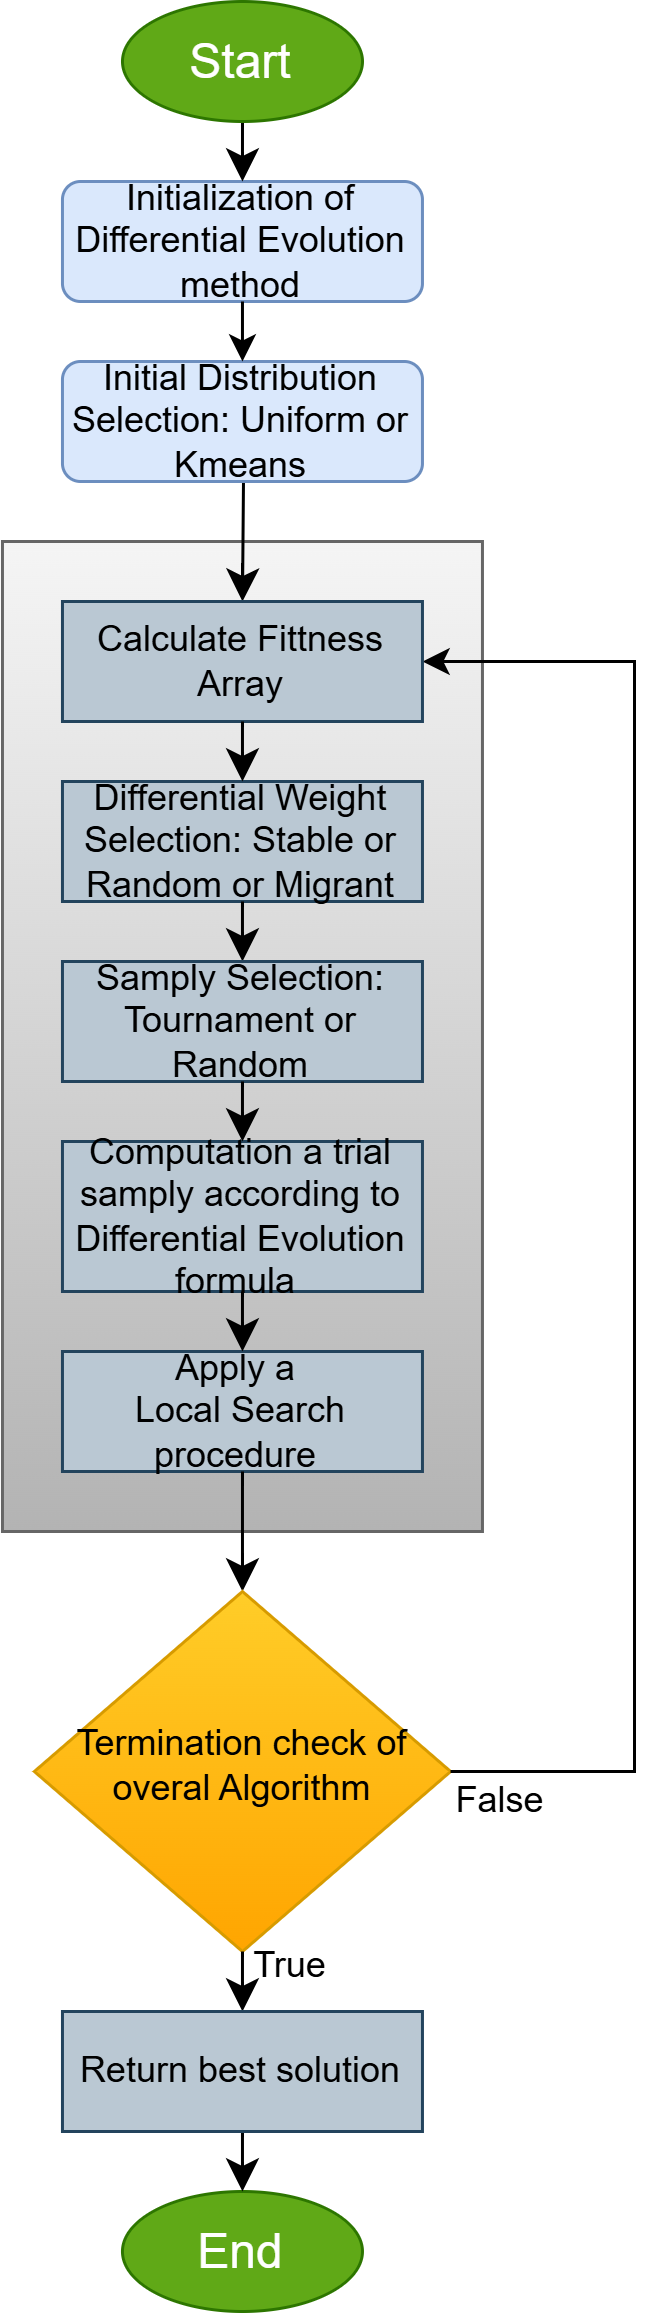
\includegraphics{flowchart}
\par\end{centering}
\caption{Flowchart of the proposed method\label{fig:FlowchartOfProposed}}

\end{figure}

The steps of the proposed Differential Evolution (DE) \ref{fig:FlowchartOfProposed}
algorithm can be described as follows:

The process begins by initializing the basic parameters, including
population size, differential weight values, and crossover probabilities.
The initial population is then generated, either uniformly distributed
over the search space or clustered using the K-means algorithm. Once
the initial population is determined, the fitness of each individual
is evaluated and stored in a fitness table. At this stage, a differential
weight calculation method is selected, with Stable, Random or Migrant
options. Likewise, the sampling procedure for generating new solutions
is specified, which may include tournament selection or random sampling.
To further refine the candidate solutions, a local search procedure
is applied, improving the quality of the trial solutions. The algorithm
then checks the termination criteria to decide whether to proceed
or terminate. If the criteria are still not met, the process returns
to update the fitness table and continues to repeat. In case the termination
criteria are met, the algorithm outputs the best solution found.

\section{Results\label{sec:Results}}

This section begins with a description of the functions that will
be used in the experiments and then presents in detail the experiments
that were performed, in which the parameters available in the proposed
algorithm were studied, in order to study its reliability and adequacy. 

\subsection{Test Functions}

A variety of test functions was used in the conducted experiments.
These functions are used in a series of research papers \citep{testfunc1,testfunc2,testfunc2-1,testfunc4}.
In the present research work, these functions were used with a varying
number of dimensions from 5 to 20. The description of each used test
function is provided below. In all cases the constant $n$ defines
the dimension of the objective function\@.
\begin{itemize}
\item F9 function, which is defined as:
\[
f(x)=-\exp\left(-0.5\sum_{i=1}^{n}x_{i}^{2}\right),\quad x\in[0,1]^{n}
\]
\item F12 function, having the following definition:
\begin{align*}
f(x) & =\frac{\pi}{n}\left(10\sin\left(\pi y_{1}\right)+\sum_{i=1}^{n-1}\left(\left(y_{i}-1\right)^{2}\left(1+10\sin^{2}\left(\pi y_{i+1}\right)\right)\right)+\left(y_{n}-1\right)^{2}\right)\\
 & +\sum_{i=1}^{n}u\left(x_{i},10,100,4\right)
\end{align*}
\item F13 function, defined as:
\[
f(x)=\sum_{i=1}^{n}\frac{x_{i}^{2}}{4000}-\prod_{i=1}^{n}\cos\left(\frac{x_{i}}{\sqrt{i}}\right)+1
\]
\item F14 function, which is defined as follows:
\[
f(x)=\left(\frac{1}{500}+\sum_{j=1}^{25}\frac{1}{j+\sum_{i=1}^{n}\left(x_{i}-a_{ij}\right)^{6}}\right)^{-1}
\]
\item F15 function, with the following definition
\[
f(x)=\sum_{i=1}^{11}\left(a_{i}-\frac{x_{1}\left(b_{i}+b_{i}x_{2}\right)}{b_{i}^{2}+b_{i}x_{3}+x_{4}}\right)^{2}
\]
\item F18 function, which has the following definition
\[
f(x)=-\sum_{i=1}^{4}c_{1}\exp\left(-\sum_{j=1}^{n}a_{ij}\left(x_{j}-p_{ij}\right)^{2}\right)
\]
where $c_{1}=0.965$
\item F19 function, defined as
\[
f(x)=-\sum_{i=1}^{4}c_{1}\exp\left(-\sum_{j=1}^{n}a_{ij}\left(x_{j}-p_{ij}\right)^{2}\right)
\]
where $c_{1}=0.83$
\item TEST2N function, with the following definition:
\[
f(x)=\frac{1}{2}\sum_{i=1}^{n}x_{i}^{4}-16x_{i}^{2}+5x_{i},\quad x_{i}\in[-5,5].
\]
\item ELP function, with the following definition:
\[
f(x)=\sum_{i=1}^{n}\left(10^{6}\right)^{\frac{i-1}{n-1}}x_{i}^{2}
\]
\item SCHWEFEL221 function, defined as
\[
f(x)=418.9829n+\sum_{i=1}^{n}-x_{i}\sin\left(\sqrt{\left|x_{i}\right|}\right)
\]
\item SINU function defined as:
\[
f(x)=-\left(2.5\prod_{i=1}^{n}\sin\left(x_{i}-z\right)+\prod_{i=1}^{n}\sin\left(5\left(x_{i}-z\right)\right)\right),\quad0\le x_{i}\le\pi.
\]
\end{itemize}

\subsection{Experimental results }

A series of experiments was carried out for the previously mentioned
functions and these experiments were executed on an AMD RYZEN 5950X
with 128GB RAM. The operating system of the running machine was Debian
Linux. Each experiment was conducted 30 times, with different random
numbers each time, and the averages were recorded. The software used
in the experiments was coded in ANSI C++ using the freely available
optimization environment of OPTIMUS, which can be downloaded from\textbf{
}\url{https://github.com/itsoulos/OPTIMUS} (accessed on 11 December
2024). The values for the experimental parameters used in the proposed
method are outlined in Table \ref{tab:expSettings}. 

\begin{table}[H]
\caption{The values of the parameters of the proposed method.\label{tab:expSettings}}

\centering{}%
\begin{tabular}{|c|c|c|}
\hline 
PARAMETER & MEANING & VALUE\tabularnewline
\hline 
\hline 
$NP$ & Number of agents & 200\tabularnewline
\hline 
$p_{l}$ & Local search rate & 0.01\tabularnewline
\hline 
$F$ & Differential weight & 0.8\tabularnewline
\hline 
$CR$ & Crossover probability & 0.9\tabularnewline
\hline 
$N_{g}$ & Maximum number of allowed iterations & 200\tabularnewline
\hline 
$N_{I}$ & Number of iterations used in the termination rule & 10\tabularnewline
\hline 
$N_{t}$ & Tournament size & 8\tabularnewline
\hline 
\end{tabular}
\end{table}
In the following tables that depict the experimental results, the
numbers in cells stand for the average function calls, as measured
on 30 independent runs. The numbers in parentheses denote the fraction
of the executions where the method discovered successfully the global
minimum. If this number is not present, then the method managed to
locate the global minimum in every run ( 100\% success).

\subsection{The proposed method in comparison with others}

The comparison of the results for four large scale optimization methods
(AQUILA, AOA, SAO, and PROPOSED) is based on a set of test functions
with varying dimensions (5, 10, 15, and 20). The measurements include
the number of objective function evaluations and the corresponding
success rates, as detailed in the Table \ref{tab:MainComparison}.
The overall performance of the methods, in terms of objective function
evaluations, reveals significant differences. The AQUILA method \citep{key-1-2}recorded
a total of 1,964,278 evaluations, while AOA\citep{key-2-2} reached
1,967,295 evaluations, representing the highest number of calls among
the four methods. The SAO method\citep{key-4-1} required 1,931,008
evaluations, the lowest among the first three methods. On the other
hand, the PROPOSED method achieved substantially fewer evaluations,
with only 435,161 calls in total. This stark difference highlights
the computational efficiency of the PROPOSED method, which requires
significantly fewer evaluations to achieve convergence compared to
the other methods. The effectiveness of each method was also evaluated
based on their success rates. AQUILA achieved an average success rate
of 91\%, AOA 92\%, and SAO 90\%, while the PROPOSED method achieved
the highest average success rate of 93\%. Despite its lower computational
cost, the PROPOSED method demonstrates remarkable reliability by achieving
the highest success rate among all methods. An analysis based on function
dimensionality shows that all methods perform well for lower dimensions
(5 and 10). However, as the dimensionality increases (15 and 20),
differences emerge. The PROPOSED method continues to exhibit high
efficiency even at higher dimensions, such as for functions F12 and
F14 in dimensions 15 and 20, where the success rate remains above
76\%. AQUILA, AOA, and SAO maintain consistently high success rates
regardless of dimensionality but at a higher computational cost. For
challenging functions such as TEST2N and SCHWEFEL221, the PROPOSED
method achieves significantly lower objective function evaluations
compared to the other methods without sacrificing success rates. For
instance, in the case of TEST2N with a dimension of 20, the PROPOSED
method achieves a success rate of 93.33\% with only 9,686 evaluations,
while the other methods require tens of thousands of evaluations to
converge. Overall, the PROPOSED method clearly outperforms the others
in terms of objective function evaluations, achieving exceptionally
low values compared to its counterparts. At the same time, it maintains
the highest average success rate, demonstrating its ability to deliver
effective and reliable results with minimal computational cost. Furthermore,
the PROPOSED method proves to be resilient to increased dimensionality,
maintaining satisfactory success rates while remaining highly efficient.
For more challenging functions, such as TEST2N and SCHWEFEL221, the
PROPOSED method stands out as the most efficient, with a significant
reduction in the required number of evaluations. The PROPOSED method
emerges as a highly promising approach, combining high accuracy with
a significant reduction in computational cost. This makes it an ideal
choice for applications where limited computational resources are
a critical consideration.

\begin{table}
\caption{Comparison of function calls and success rates of proposed method
against others\label{tab:MainComparison}}

\begin{centering}
\begin{tabular}{|c|c|c|c|c|c|}
\hline 
\textbf{FUNCTION} & \textbf{DIM} & \textbf{AQUILA} & \textbf{AOA} & \textbf{SAO} & \textbf{PROPOSED}\tabularnewline
\hline 
\hline 
F9 & 5 & 44104 & 40761 & 42057 & 13232\tabularnewline
\hline 
F9 & 10 & 58929 & 53564 & 55360 & 46006\tabularnewline
\hline 
F9 & 15 & 66786 & 61764 & 62149 & 79489\tabularnewline
\hline 
F9 & 20 & 73446 & 64223 & 65948 & 96174\tabularnewline
\hline 
F12 & 5 & 29168 & 29362 & 29020 & 3538(0.97)\tabularnewline
\hline 
F12 & 10 & 46769 & 47141 & 44627 & 4332\tabularnewline
\hline 
F12 & 15 & 53808 & 56265 & 51916 & 5050\tabularnewline
\hline 
F12 & 20 & 58314 & 60502 & 55332 & 5477(0.97)\tabularnewline
\hline 
F13 & 5 & 30506 & 31091 & 31070 & 2367\tabularnewline
\hline 
F13 & 10 & 39429 & 40174 & 40111 & 4336\tabularnewline
\hline 
F13 & 15 & 43704 & 45253 & 44298 & 5036\tabularnewline
\hline 
F13 & 20 & 45506 & 47368 & 46021 & 5265\tabularnewline
\hline 
F14 & 5 & 32845 & 33677 & 34005 & 3061\tabularnewline
\hline 
F14 & 10 & 43539 & 43191 & 43462 & 4293\tabularnewline
\hline 
F14 & 15 & 46336 & 46316 & 45866 & 5877(0.84)\tabularnewline
\hline 
F14 & 20 & 53625 & 52626 & 51437 & 6362(0.77)\tabularnewline
\hline 
F15 & 5 & 35396 & 37502 & 36273 & 3256(0.50)\tabularnewline
\hline 
F15 & 10 & 50030 & 52312 & 49821 & 4775(0.94)\tabularnewline
\hline 
F15 & 15 & 57247 & 58773 & 56417 & 5371(0.97)\tabularnewline
\hline 
F15 & 20 & 59520 & 60608 & 58880 & 5887\tabularnewline
\hline 
F18 & 5 & 27263 & 27262 & 27272 & 1598\tabularnewline
\hline 
F18 & 10 & 35707 & 35725 & 35710 & 2092\tabularnewline
\hline 
F18 & 15 & 38811 & 38816 & 38796 & 2271\tabularnewline
\hline 
F18 & 20 & 40230 & 40237 & 40253 & 2354\tabularnewline
\hline 
F19 & 5 & 27547 & 27539 & 27546 & 1613\tabularnewline
\hline 
F19 & 10 & 35970 & 35965 & 35981 & 2106\tabularnewline
\hline 
F19 & 15 & 39101 & 39118 & 39107 & 2291\tabularnewline
\hline 
F19 & 20 & 40485 & 40493 & 40484 & 2370\tabularnewline
\hline 
TEST2N & 5 & 31914 & 32617 & 32206 & 3860\tabularnewline
\hline 
TEST2N & 10 & 44773(0.90) & 45276 & 44868(0.30) & 6314(0.94)\tabularnewline
\hline 
TEST2N & 15 & 52404(0.17) & 52731(0.54) & 52133(0.10) & 8224\tabularnewline
\hline 
TEST2N & 20 & 56242(0.03) & 56237(0.10) & 55680(0.06) & 9686(0.94)\tabularnewline
\hline 
ELP & 5 & 30806 & 30525 & 30339 & 3378\tabularnewline
\hline 
ELP & 10 & 43720 & 42910 & 42700 & 5448\tabularnewline
\hline 
ELP & 15 & 51582 & 50692 & 50096 & 7033\tabularnewline
\hline 
ELP & 20 & 56392 & 55278 & 54398 & 8292\tabularnewline
\hline 
SCHWEFEL221 & 5 & 28086 & 28168 & 28153 & 3431\tabularnewline
\hline 
SCHWEFEL221 & 10 & 40901 & 40757 & 40074 & 4446\tabularnewline
\hline 
SCHWEFEL221 & 15 & 47139(0.06) & 47191(0.03) & 46865(0.10) & 13216(0.06)\tabularnewline
\hline 
SCHWEFEL221 & 20 & 49987(0.03) & 50476(0.03) & 49415(0.03) & 15301(0.20)\tabularnewline
\hline 
SINU & 5 & 31234 & 32816 & 32684 & 3519\tabularnewline
\hline 
SINU & 10 & 42244 & 44754 & 43473 & 4948\tabularnewline
\hline 
SINU & 15 & 49064 & 52019 & 47896 & 5847\tabularnewline
\hline 
SINU & 20 & 53669 & 57220 & 50809 & 6339\tabularnewline
\hline 
\textbf{TOTAL} &  & \textbf{1964278} & \textbf{1967295} & \textbf{1931008} & \textbf{435161}\tabularnewline
\hline 
\end{tabular}
\par\end{centering}
\end{table}

Figure \ref{fig:StatisticalMainComp} was generated by executing a
script in R, which applied the Friedman test for statistical analysis,
based on Table \ref{tab:MainComparison}. The table includes the objective
function calls for the four optimization methods (AQUILA, AOA, SAO,
and PROPOSED), excluding the columns related to success rates. The
aim of the analysis was to investigate the presence of statistically
significant differences among the methods, with a particular focus
on evaluating the performance of the proposed method (PROPOSED) compared
to the others. The results of the Friedman test revealed the presence
of highly significant differences (p-value \textless{} 0.0001) in
all pairwise comparisons between the proposed method and the other
three. This indicates that the proposed method is statistically superior
to AQUILA, AOA, and SAO in terms of efficiency, as reflected by the
number of required objective function calls. The proposed method demonstrated
significantly lower values in objective function calls compared to
the other three methods. This suggests that PROPOSED is clearly more
efficient, achieving convergent solutions with substantially reduced
computational cost. The statistical analysis confirms that these differences
are not due to random effects but are systematic and reproducible.
Furthermore, the pairwise comparisons highlighted that the PROPOSED
method outperforms even in cases where the other methods exhibit high
stability in their calls, such as for functions with lower dimensions.
Specifically, for more complex functions or those with higher dimensions,
the superiority of the proposed method becomes even more pronounced,
reinforcing its position as a more efficient and suitable choice for
such cases. The statistical significance revealed through the Friedman
test provides an objective basis for concluding that the proposed
method offers not only high accuracy and reliability but also significantly
lower computational cost. The analysis further underscores the value
of PROPOSED as an innovative and improved approach to optimization
methods.

\begin{figure}
\begin{centering}
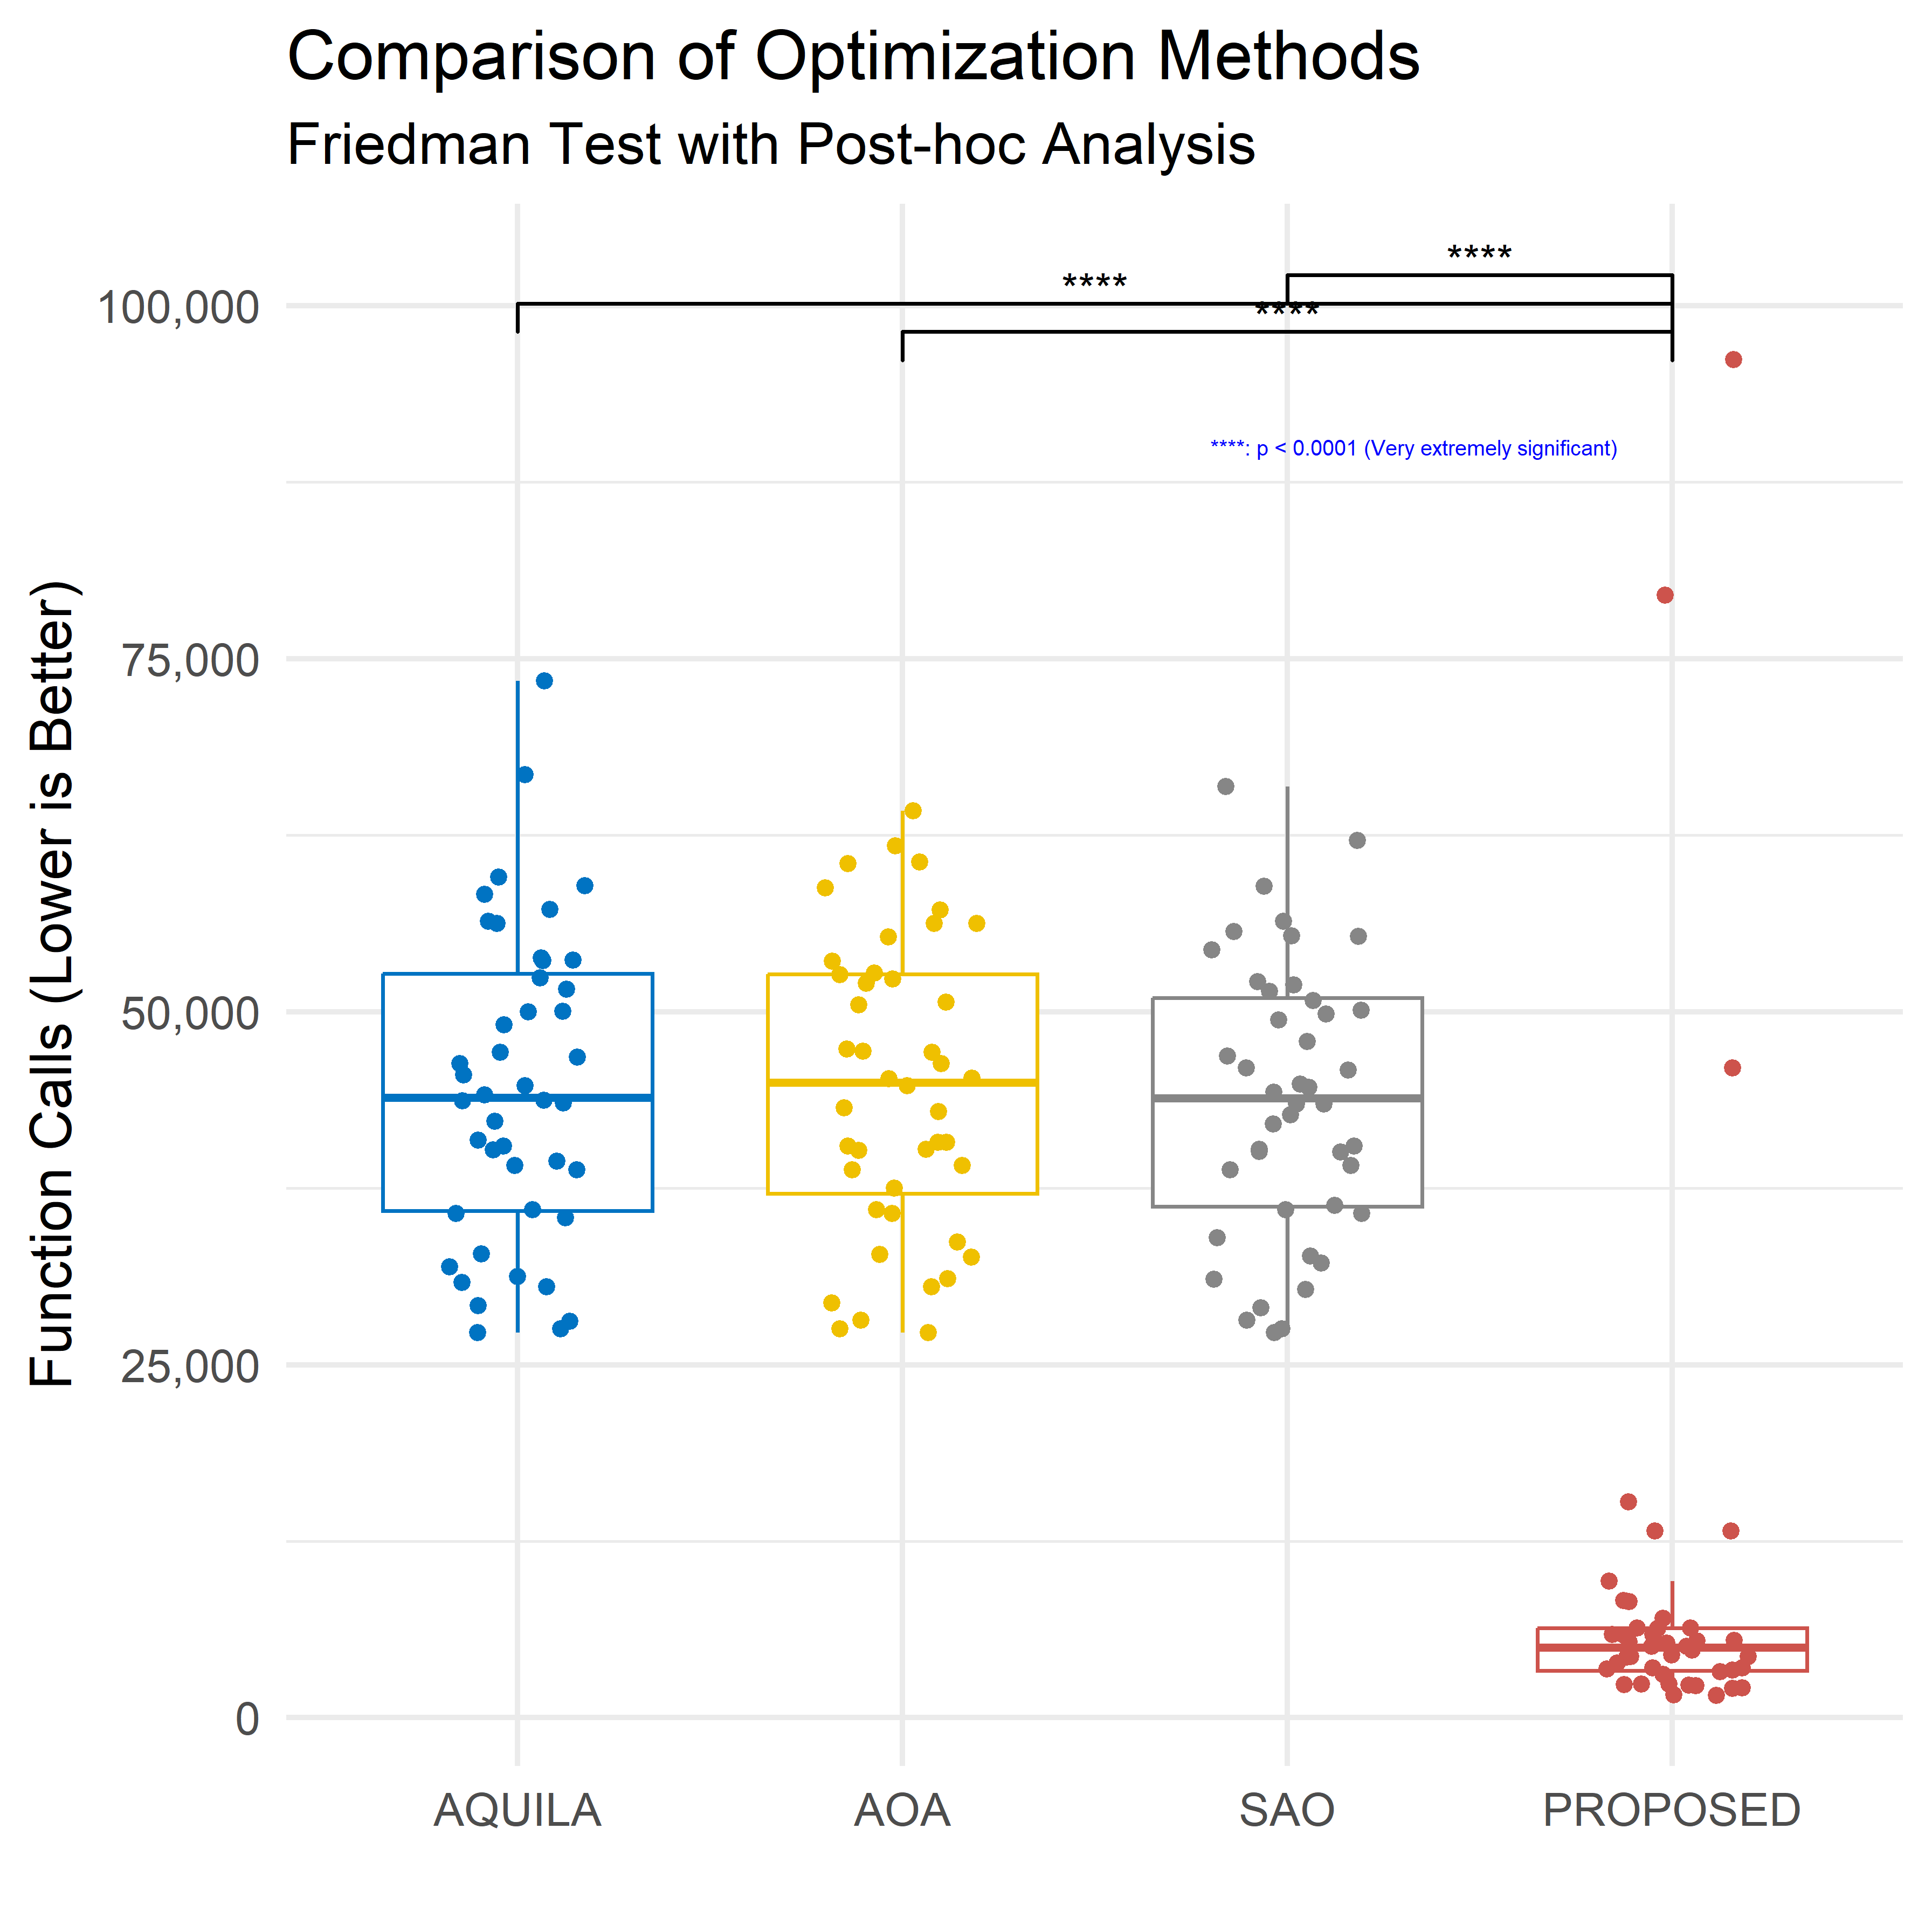
\includegraphics[scale=0.5]{friedmanMethodsCalls}\caption{Statistical comparison of function calls of proposed method against
others\label{fig:StatisticalMainComp} }
\par\end{centering}
\end{figure}


\subsection{The effect of differential weight mechanism}

The table \ref{tab:expWeight} presents the objective function evaluations
required by the differential evolution method for different test functions
and dimensions. It is noted that the sample selection in the basic
differential evolution framework is random. Three approaches for calculating
the differential weight are compared: constant value, random selection,
and the MIGRANT approach. The values in parentheses indicate the success
rate of each approach (e.g., 0.97 corresponds to 97\%). In all cases,
the initial sample distribution was uniform. The analysis of the results
shows that the number of objective function evaluations generally
increases with the dimension for all test functions. For example,
in the F9 function, the evaluations increase from 69034 in dimension
5 to 75942 in dimension 20 when the differential weight is constant.
Similar trends are observed in the other two approaches, with the
MIGRANT approach generally requiring fewer evaluations, especially
in higher dimensions. The performance of the MIGRANT approach varies
depending on the function and the dimension. For instance, in the
F15 function with dimension 20, MIGRANT records 6145 evaluations with
a success rate of 0.97, a significantly lower number of evaluations
compared to the other two approaches. Conversely, in the F13 function
for dimension 20, relatively low success rates are observed (0.37
for the MIGRANT approach versus 0.63 when the differential weight
is constant). The average number of evaluations for the three approaches
is 931043 for a constant differential weight, 825891 for random selection,
and 445122 for the MIGRANT approach. The success rates are similar
across the approaches, with values of 0.82, 0.83, and 0.81, respectively.
However, the MIGRANT approach demonstrates greater efficiency in several
cases, achieving comparable or even higher success rates with significantly
fewer evaluations. Specific functions such as TEST2N and F15 clearly
show the superiority of MIGRANT, as this approach achieves high success
rates (up to 0.97) with a reduced number of evaluations. Similarly,
in the SCHWEFEL221 function, MIGRANT shows better efficiency for higher
dimensions, with an example of 14832 evaluations in dimension 20 compared
to 58552 when the differential weight is constant. In conclusion,
MIGRANT emerges as an approach that offers competitive advantages
over the other two, especially in higher-dimensional problems. The
choice of the appropriate approach depends on the problem requirements
and the complexity of the test function.

\begin{table}[H]
\caption{Comparing different differential weight mechanisms.\label{tab:expWeight}}

\centering{}{\footnotesize{}}%
\begin{tabular}{|c|c|c|c|c|}
\hline 
{\footnotesize{}FUNCTION} & {\footnotesize{}DIM} & {\footnotesize{}NUMBER(R)} & {\footnotesize{}RANDOM(R)} & {\footnotesize{}MIGRANT(R)}\tabularnewline
\hline 
\hline 
{\footnotesize{}F9} & {\footnotesize{}5} & {\footnotesize{}69034} & {\footnotesize{}68262} & {\footnotesize{}9336(0.57)}\tabularnewline
\hline 
{\footnotesize{}F9} & {\footnotesize{}10} & {\footnotesize{}73049(0.03)} & {\footnotesize{}72599(0.03)} & {\footnotesize{}54467(0.03)}\tabularnewline
\hline 
{\footnotesize{}F9} & {\footnotesize{}15} & {\footnotesize{}73795(0.03)} & {\footnotesize{}73312(0.03)} & {\footnotesize{}73491(0.03)}\tabularnewline
\hline 
{\footnotesize{}F9} & {\footnotesize{}20} & {\footnotesize{}75942(0.03)} & {\footnotesize{}75189(0.03)} & {\footnotesize{}75711(0.03)}\tabularnewline
\hline 
{\footnotesize{}F12} & {\footnotesize{}5} & {\footnotesize{}9715} & {\footnotesize{}7986} & {\footnotesize{}5057}\tabularnewline
\hline 
{\footnotesize{}F12} & {\footnotesize{}10} & {\footnotesize{}12219} & {\footnotesize{}9559} & {\footnotesize{}4991}\tabularnewline
\hline 
{\footnotesize{}F12} & {\footnotesize{}15} & {\footnotesize{}14101} & {\footnotesize{}11027} & {\footnotesize{}5428}\tabularnewline
\hline 
{\footnotesize{}F12} & {\footnotesize{}20} & {\footnotesize{}18282} & {\footnotesize{}14090} & {\footnotesize{}5845}\tabularnewline
\hline 
{\footnotesize{}F13} & {\footnotesize{}5} & {\footnotesize{}5759(0.03)} & {\footnotesize{}5274(0.03)} & {\footnotesize{}3700(0.03)}\tabularnewline
\hline 
{\footnotesize{}F13} & {\footnotesize{}10} & {\footnotesize{}22947(0.03)} & {\footnotesize{}15072(0.03)} & {\footnotesize{}5219(0.03)}\tabularnewline
\hline 
{\footnotesize{}F13} & {\footnotesize{}15} & {\footnotesize{}20102(0.03)} & {\footnotesize{}17305(0.03)} & {\footnotesize{}5478(0.07)}\tabularnewline
\hline 
{\footnotesize{}F13} & {\footnotesize{}20} & {\footnotesize{}14189(0.63)} & {\footnotesize{}13606(0.50)} & {\footnotesize{}5482(0.37)}\tabularnewline
\hline 
{\footnotesize{}F14} & {\footnotesize{}5} & {\footnotesize{}7001} & {\footnotesize{}6346} & {\footnotesize{}4779}\tabularnewline
\hline 
{\footnotesize{}F14} & {\footnotesize{}10} & {\footnotesize{}7953} & {\footnotesize{}7082} & {\footnotesize{}5085}\tabularnewline
\hline 
{\footnotesize{}F14} & {\footnotesize{}15} & {\footnotesize{}15165} & {\footnotesize{}11991} & {\footnotesize{}6455(0.93)}\tabularnewline
\hline 
{\footnotesize{}F14} & {\footnotesize{}20} & {\footnotesize{}13338} & {\footnotesize{}11690} & {\footnotesize{}6192(0.93)}\tabularnewline
\hline 
{\footnotesize{}F15} & {\footnotesize{}5} & {\footnotesize{}7917} & {\footnotesize{}7181(0.83)} & {\footnotesize{}4996(0.70)}\tabularnewline
\hline 
{\footnotesize{}F15} & {\footnotesize{}10} & {\footnotesize{}9155} & {\footnotesize{}8361} & {\footnotesize{}5537(0.97)}\tabularnewline
\hline 
{\footnotesize{}F15} & {\footnotesize{}15} & {\footnotesize{}10473} & {\footnotesize{}9122} & {\footnotesize{}5909(0.97)}\tabularnewline
\hline 
{\footnotesize{}F15} & {\footnotesize{}20} & {\footnotesize{}11650} & {\footnotesize{}9729} & {\footnotesize{}6145(0.97)}\tabularnewline
\hline 
{\footnotesize{}F18} & {\footnotesize{}5} & {\footnotesize{}2443} & {\footnotesize{}2446} & {\footnotesize{}2424}\tabularnewline
\hline 
{\footnotesize{}F18} & {\footnotesize{}10} & {\footnotesize{}2445} & {\footnotesize{}2448} & {\footnotesize{}2422}\tabularnewline
\hline 
{\footnotesize{}F18} & {\footnotesize{}15} & {\footnotesize{}2447} & {\footnotesize{}2446} & {\footnotesize{}2311}\tabularnewline
\hline 
{\footnotesize{}F18} & {\footnotesize{}20} & {\footnotesize{}2545} & {\footnotesize{}2448} & {\footnotesize{}2402}\tabularnewline
\hline 
{\footnotesize{}F19} & {\footnotesize{}5} & {\footnotesize{}2403} & {\footnotesize{}2612} & {\footnotesize{}2402}\tabularnewline
\hline 
{\footnotesize{}F19} & {\footnotesize{}10} & {\footnotesize{}2643} & {\footnotesize{}2602} & {\footnotesize{}2532}\tabularnewline
\hline 
{\footnotesize{}F19} & {\footnotesize{}15} & {\footnotesize{}2596} & {\footnotesize{}2593} & {\footnotesize{}2922}\tabularnewline
\hline 
{\footnotesize{}F19} & {\footnotesize{}20} & {\footnotesize{}2673} & {\footnotesize{}2459} & {\footnotesize{}2611}\tabularnewline
\hline 
{\footnotesize{}TEST2N} & {\footnotesize{}5} & {\footnotesize{}16355} & {\footnotesize{}12978} & {\footnotesize{}5602}\tabularnewline
\hline 
{\footnotesize{}TEST2N} & {\footnotesize{}10} & {\footnotesize{}35647} & {\footnotesize{}27151} & {\footnotesize{}7245}\tabularnewline
\hline 
{\footnotesize{}TEST2N} & {\footnotesize{}15} & {\footnotesize{}56031} & {\footnotesize{}46514} & {\footnotesize{}8586(0.93)}\tabularnewline
\hline 
{\footnotesize{}TEST2N} & {\footnotesize{}20} & {\footnotesize{}66045} & {\footnotesize{}65758} & {\footnotesize{}10108(0.83)}\tabularnewline
\hline 
{\footnotesize{}ELP} & {\footnotesize{}5} & {\footnotesize{}11978} & {\footnotesize{}10846} & {\footnotesize{}5176}\tabularnewline
\hline 
{\footnotesize{}ELP} & {\footnotesize{}10} & {\footnotesize{}15048} & {\footnotesize{}14546} & {\footnotesize{}6555}\tabularnewline
\hline 
{\footnotesize{}ELP} & {\footnotesize{}15} & {\footnotesize{}17190} & {\footnotesize{}17170} & {\footnotesize{}7758}\tabularnewline
\hline 
{\footnotesize{}ELP} & {\footnotesize{}20} & {\footnotesize{}19063} & {\footnotesize{}19349} & {\footnotesize{}8880}\tabularnewline
\hline 
{\footnotesize{}SCHWEFEL221} & {\footnotesize{}5} & {\footnotesize{}8048} & {\footnotesize{}7210} & {\footnotesize{}4918}\tabularnewline
\hline 
{\footnotesize{}SCHWEFEL221} & {\footnotesize{}10} & {\footnotesize{}13635} & {\footnotesize{}10871} & {\footnotesize{}5626}\tabularnewline
\hline 
{\footnotesize{}SCHWEFEL221} & {\footnotesize{}15} & {\footnotesize{}25843(0.07)} & {\footnotesize{}27354(0.07)} & {\footnotesize{}13895(0.30)}\tabularnewline
\hline 
{\footnotesize{}SCHWEFEL221} & {\footnotesize{}20} & {\footnotesize{}58552(0.20)} & {\footnotesize{}57631(0.70)} & {\footnotesize{}14832(0.70)}\tabularnewline
\hline 
{\footnotesize{}SINU} & {\footnotesize{}5} & {\footnotesize{}12886} & {\footnotesize{}9938} & {\footnotesize{}5280}\tabularnewline
\hline 
{\footnotesize{}SINU} & {\footnotesize{}10} & {\footnotesize{}16103} & {\footnotesize{}13366} & {\footnotesize{}5992}\tabularnewline
\hline 
{\footnotesize{}SINU} & {\footnotesize{}15} & {\footnotesize{}20535} & {\footnotesize{}17018} & {\footnotesize{}7209}\tabularnewline
\hline 
{\footnotesize{}SINU} & {\footnotesize{}20} & {\footnotesize{}26103} & {\footnotesize{}20354} & {\footnotesize{}8601}\tabularnewline
\hline 
\textbf{\footnotesize{}AVERAGE} &  & \textbf{\footnotesize{}931043(0.82)} & \textbf{\footnotesize{}825891(0.83)} & \textbf{\footnotesize{}445122(0.81)}\tabularnewline
\hline 
\end{tabular}{\footnotesize\par}
\end{table}

In figure \ref{fig:statWeight}, the overall analysis, which includes
all pairwise comparisons, yielded a p-value of 1.1e-05. This value
is significantly smaller than the conventional significance level
(p=0.05), indicating that there are clear statistically significant
differences among the groups. This result suggests that the compared
techniques do not exhibit homogeneity and that the observed differences
in outcomes are unlikely to be due to chance. The comparison between
the NUMBER(R) and RANDOM(R) methods produced a p-value of 1.5e-05.
This value is similarly very small, signifying that these two methods
display statistically significant differences. For the comparison
of NUMBER(R) with MIGRANT(R), the p-value was also 1.5e-05. This finding
confirms that these two methods also exhibit significantly different
performance characteristics. The statistical significance observed
here underscores that the differences in results between NUMBER(R)
and MIGRANT(R) cannot be ignored. The final pairwise comparison, between
RANDOM(R) and MIGRANT(R), yielded a p-value of 1e-04. Although this
value is larger than the previous ones, it is still well below the
significance threshold of p=0.05. Therefore, in this case as well,
statistically significant differences between the two approaches are
evident, indicating variations in their effectiveness or the stability
of their results. Overall, the very low p-values obtained from all
comparisons point to clear and systematic differences among the methods.
This indicates that each approach has distinct characteristics that
set it apart from the others, whether in terms of reducing the number
of objective function evaluations or achieving high success rates.
The results of the analysis highlight the importance of selecting
the appropriate method based on the specific requirements of the problem.

\begin{figure}[H]
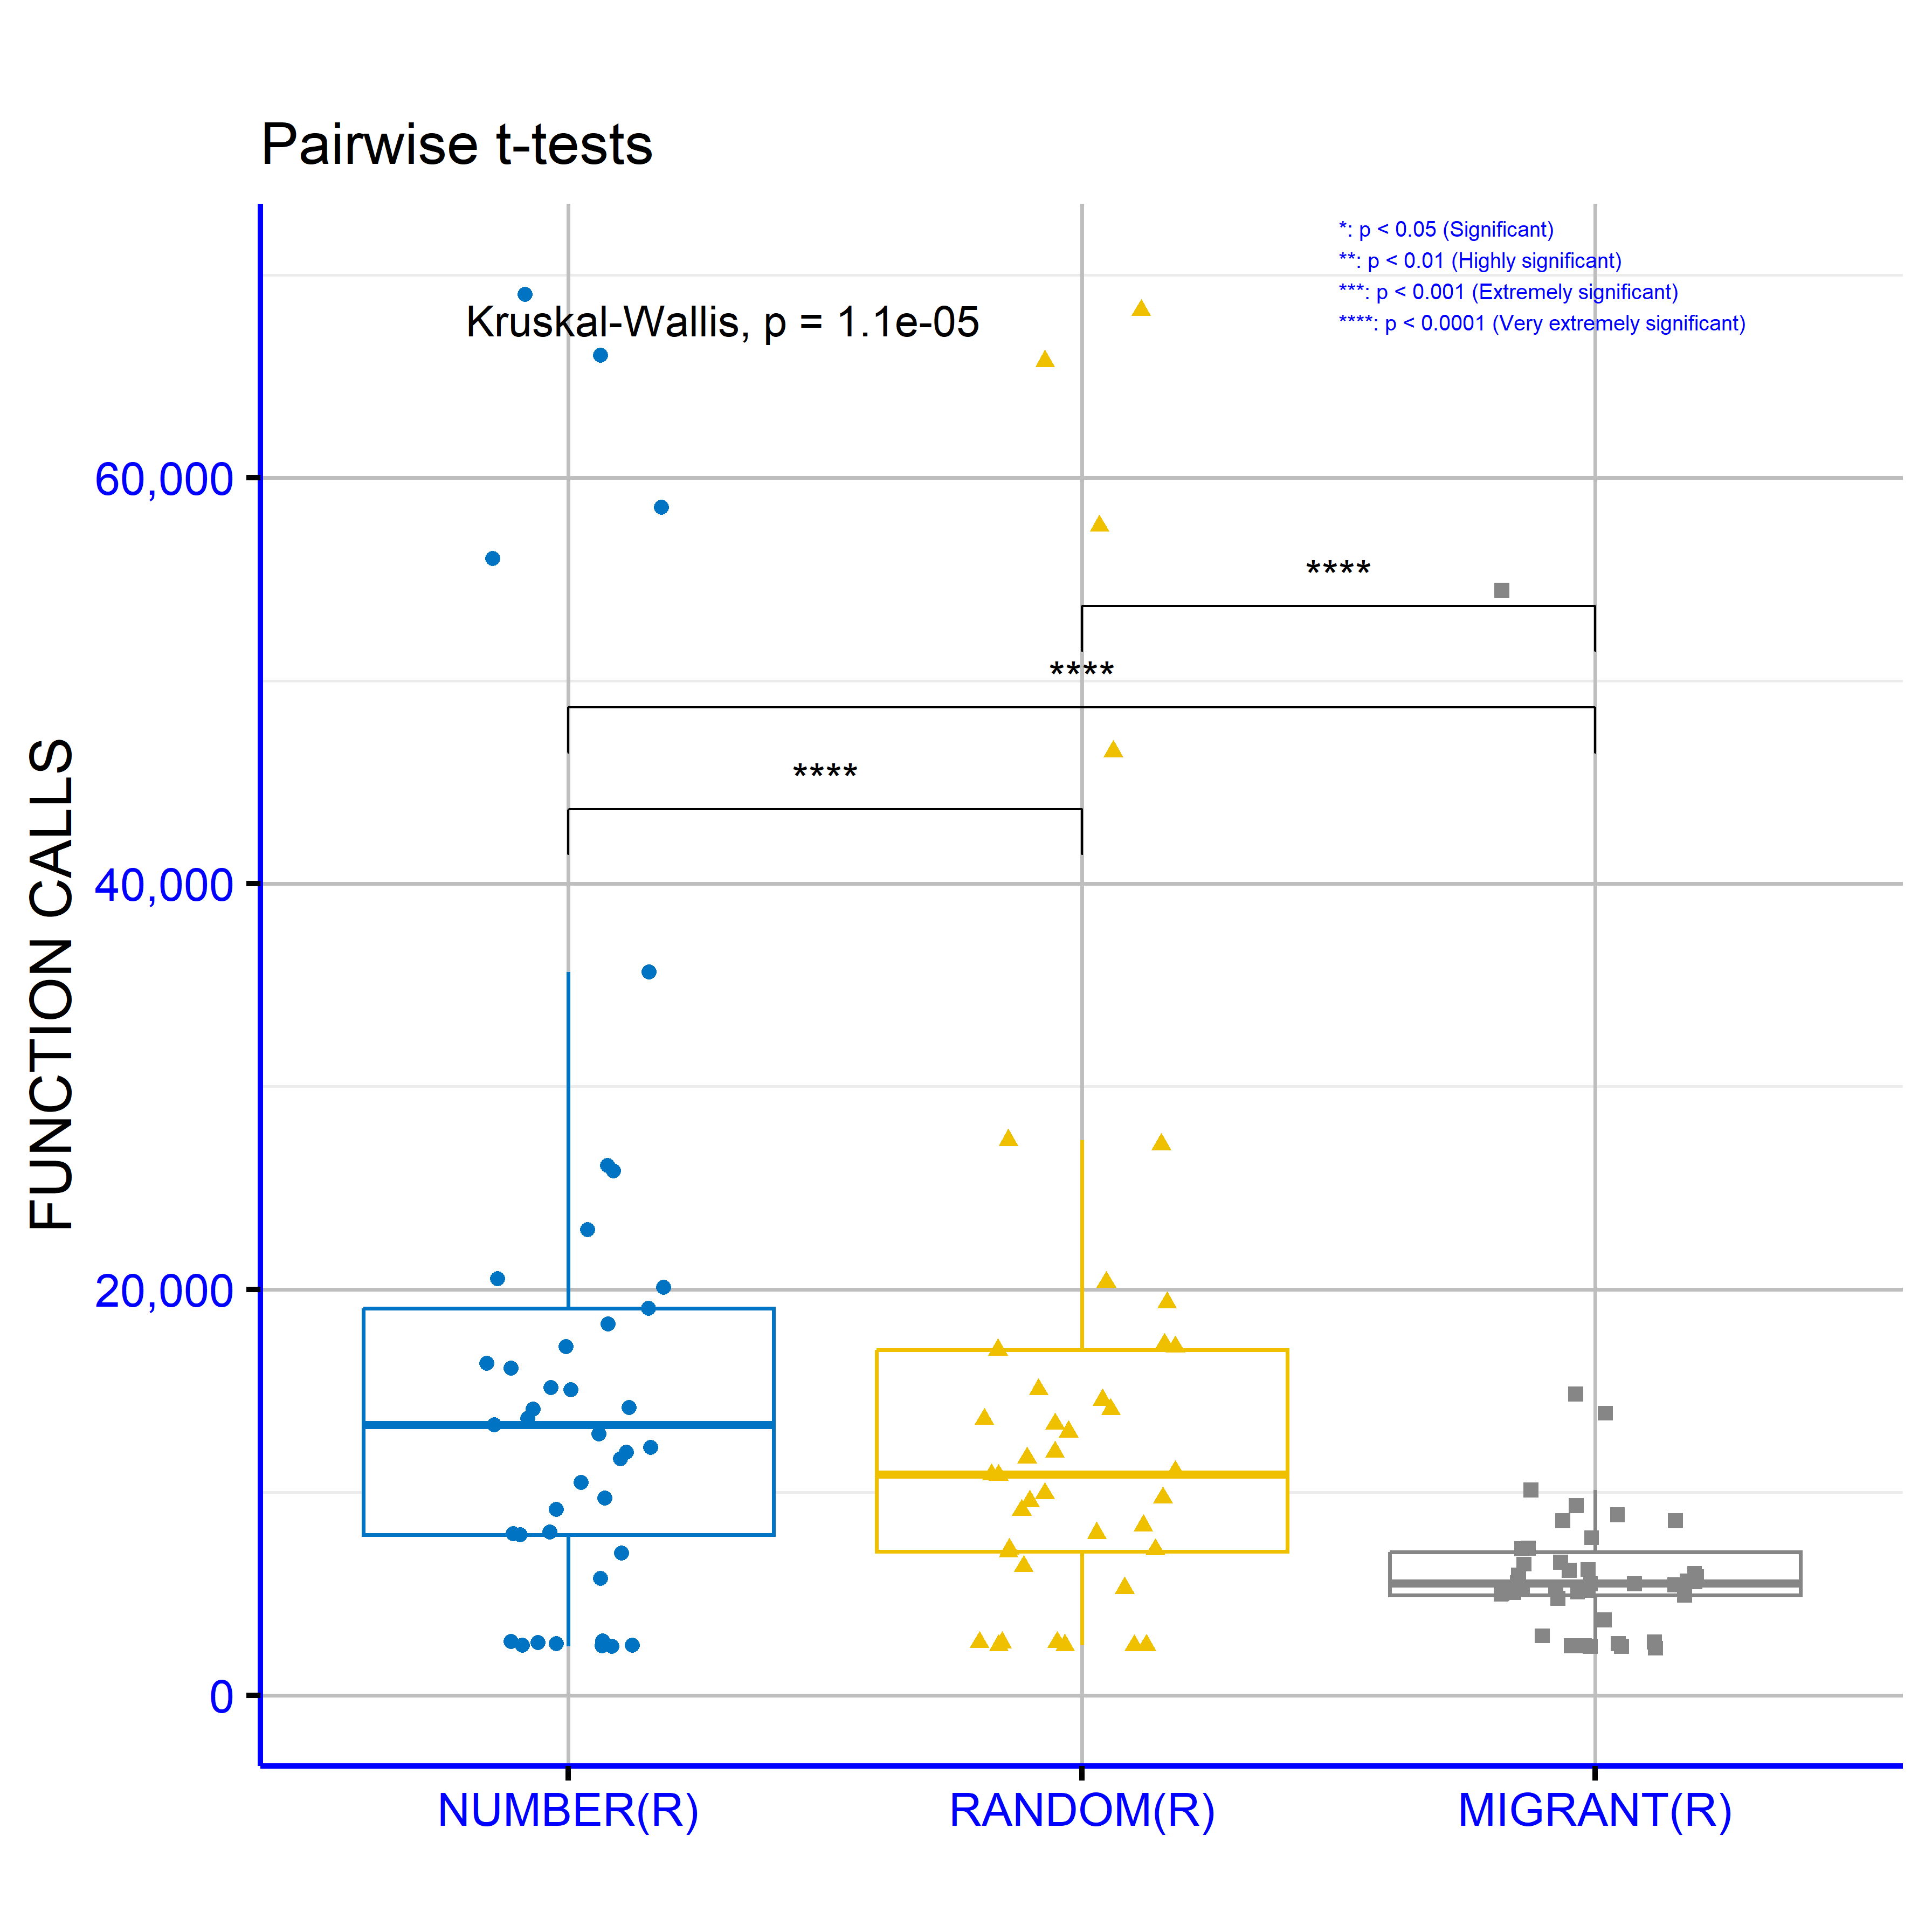
\includegraphics[scale=0.5]{stat1}
\centering{}\caption{Statistical comparison between the different variations of the proposed
method for the series of objective problems.\label{fig:statWeight}}
\end{figure}


\subsection{The effect of selection mechanism}

Table \ref{tab:selection} compares four approaches for computing
the differential weight: random differential weight with random selection
(RANDOM(R)), random differential weight with tournament selection
(RANDOM(T)), MIGRANT differential weight with random selection (MIGRANT(R)),
and MIGRANT differential weight with tournament selection (MIGRANT(T)).
Values in parentheses indicate the success rate for each approach
(e.g., 0.97 corresponds to 97\%). In all cases, the initial sample
distribution was uniform. The results analysis shows a systematic
reduction in the number of objective function evaluations when transitioning
from RANDOM(R) to MIGRANT(T). For instance, in function F9 with a
dimension of 5, the evaluations decrease from 68262 in RANDOM(R) to
4337 in MIGRANT(T), but the success rate drops significantly from
0.57 to 0.23. Similar trends are observed in other cases, where MIGRANT(T)
drastically reduces the evaluations, but the success rate is alarmingly
low in many instances. MIGRANT(T) records the lowest average number
of evaluations (186307) compared to RANDOM(R) (825891), RANDOM(T)
(503875), and MIGRANT(R) (445122). However, MIGRANT(T)’s success rate
is only 0.66, a significant disadvantage as it often fails to find
the correct solution. This success rate is much lower than the other
approaches, which maintain rates close to 0.80-0.83. Examples such
as the TEST2N function highlight the challenges of MIGRANT(T). In
dimension 20, MIGRANT(T) reduces the evaluations to 4595 compared
to 65758 for RANDOM(R), but the success rate falls to 0.10 from RANDOM(R)’s
0.93. A similar scenario occurs in the SINU function with a dimension
of 5, where MIGRANT(T) requires 3326 evaluations with a success rate
of 0.77, compared to RANDOM(R)’s 9938 evaluations but with higher
reliability (success rate of 1.0). It is essential to note that despite
the reduction in evaluations, MIGRANT(T) is particularly ineffective
when solution accuracy is a priority. Applications requiring high
accuracy (i.e., high success rates) will face significant challenges
with this approach, limiting its usability to specific problem domains.
In conclusion, MIGRANT(T) offers remarkable reductions in the number
of evaluations, but its very low success rate (66\% on average) is
a major drawback. This makes it less suitable for scenarios where
solution reliability is critical, even though the reduction in evaluations
is impressive. Its selection should be made cautiously, depending
on the problem’s requirements.

\begin{table}[H]
\caption{Experimental results comparing random and tournament selection.\label{tab:selection}}

\centering{}{\footnotesize{}}%
\begin{tabular}{|c|c|c|c|c|c|}
\hline 
{\footnotesize{}FUNCTION} & {\footnotesize{}DIM} & {\footnotesize{}RANDOM(R)} & {\footnotesize{}RANDOM(T)} & {\footnotesize{}MIGRANT(R)} & {\footnotesize{}MIGRANT(T)}\tabularnewline
\hline 
\hline 
{\footnotesize{}F9} & {\footnotesize{}5} & {\footnotesize{}68262} & {\footnotesize{}67178} & {\footnotesize{}9336(0.57)} & {\footnotesize{}4337(0.23)}\tabularnewline
\hline 
{\footnotesize{}F9} & {\footnotesize{}10} & {\footnotesize{}72599(0.03)} & {\footnotesize{}71680(0.03)} & {\footnotesize{}54467(0.03)} & {\footnotesize{}8156(0.03)}\tabularnewline
\hline 
{\footnotesize{}F9} & {\footnotesize{}15} & {\footnotesize{}73312(0.03)} & {\footnotesize{}75608(0.03)} & {\footnotesize{}73491(0.03)} & {\footnotesize{}13156(0.03)}\tabularnewline
\hline 
{\footnotesize{}F9} & {\footnotesize{}20} & {\footnotesize{}75189(0.03)} & {\footnotesize{}75827(0.03)} & {\footnotesize{}75711(0.03)} & {\footnotesize{}19711(0.03)}\tabularnewline
\hline 
{\footnotesize{}F12} & {\footnotesize{}5} & {\footnotesize{}7986} & {\footnotesize{}4085} & {\footnotesize{}5057} & {\footnotesize{}3366(0.90)}\tabularnewline
\hline 
{\footnotesize{}F12} & {\footnotesize{}10} & {\footnotesize{}9559} & {\footnotesize{}4113} & {\footnotesize{}4991} & {\footnotesize{}3135}\tabularnewline
\hline 
{\footnotesize{}F12} & {\footnotesize{}15} & {\footnotesize{}11027} & {\footnotesize{}4367} & {\footnotesize{}5428} & {\footnotesize{}3246(0.97)}\tabularnewline
\hline 
{\footnotesize{}F12} & {\footnotesize{}20} & {\footnotesize{}14090} & {\footnotesize{}4916} & {\footnotesize{}5845} & {\footnotesize{}3317(0.90)}\tabularnewline
\hline 
{\footnotesize{}F13} & {\footnotesize{}5} & {\footnotesize{}5274(0.03)} & {\footnotesize{}4442(0.13)} & {\footnotesize{}3700(0.03)} & {\footnotesize{}3023(0.03)}\tabularnewline
\hline 
{\footnotesize{}F13} & {\footnotesize{}10} & {\footnotesize{}15072(0.03)} & {\footnotesize{}9837(0.03)} & {\footnotesize{}5219(0.03)} & {\footnotesize{}3714(0.03)}\tabularnewline
\hline 
{\footnotesize{}F13} & {\footnotesize{}15} & {\footnotesize{}17305(0.03)} & {\footnotesize{}6425(0.03)} & {\footnotesize{}5478(0.07)} & {\footnotesize{}3823(0.03)}\tabularnewline
\hline 
{\footnotesize{}F13} & {\footnotesize{}20} & {\footnotesize{}13606(0.50)} & {\footnotesize{}5324(0.07)} & {\footnotesize{}5482(0.37)} & {\footnotesize{}3882(0.10)}\tabularnewline
\hline 
{\footnotesize{}F14} & {\footnotesize{}5} & {\footnotesize{}6346} & {\footnotesize{}3685} & {\footnotesize{}4779} & {\footnotesize{}3162}\tabularnewline
\hline 
{\footnotesize{}F14} & {\footnotesize{}10} & {\footnotesize{}7082} & {\footnotesize{}3824} & {\footnotesize{}5085} & {\footnotesize{}3319}\tabularnewline
\hline 
{\footnotesize{}F14} & {\footnotesize{}15} & {\footnotesize{}11991} & {\footnotesize{}4774(0.80)} & {\footnotesize{}6455(0.93)} & {\footnotesize{}3646(0.47)}\tabularnewline
\hline 
{\footnotesize{}F14} & {\footnotesize{}20} & {\footnotesize{}11690} & {\footnotesize{}4438} & {\footnotesize{}6192(0.93)} & {\footnotesize{}3607(0.93)}\tabularnewline
\hline 
{\footnotesize{}F15} & {\footnotesize{}5} & {\footnotesize{}7181(0.83)} & {\footnotesize{}4806(0.50)} & {\footnotesize{}4996(0.70)} & {\footnotesize{}3304(0.20)}\tabularnewline
\hline 
{\footnotesize{}F15} & {\footnotesize{}10} & {\footnotesize{}8361} & {\footnotesize{}4837(0.90)} & {\footnotesize{}5537(0.97)} & {\footnotesize{}3683(0.53)}\tabularnewline
\hline 
{\footnotesize{}F15} & {\footnotesize{}15} & {\footnotesize{}9122} & {\footnotesize{}4933(0.80)} & {\footnotesize{}5909(0.97)} & {\footnotesize{}3799(0.60)}\tabularnewline
\hline 
{\footnotesize{}F15} & {\footnotesize{}20} & {\footnotesize{}9729} & {\footnotesize{}5117} & {\footnotesize{}6145(0.97)} & {\footnotesize{}3773(0.60)}\tabularnewline
\hline 
{\footnotesize{}F18} & {\footnotesize{}5} & {\footnotesize{}2446} & {\footnotesize{}2446} & {\footnotesize{}2424} & {\footnotesize{}2425}\tabularnewline
\hline 
{\footnotesize{}F18} & {\footnotesize{}10} & {\footnotesize{}2448} & {\footnotesize{}2447} & {\footnotesize{}2422} & {\footnotesize{}2325}\tabularnewline
\hline 
{\footnotesize{}F18} & {\footnotesize{}15} & {\footnotesize{}2446} & {\footnotesize{}2450} & {\footnotesize{}2311} & {\footnotesize{}2422}\tabularnewline
\hline 
{\footnotesize{}F18} & {\footnotesize{}20} & {\footnotesize{}2448} & {\footnotesize{}2445} & {\footnotesize{}2402} & {\footnotesize{}2511}\tabularnewline
\hline 
{\footnotesize{}F19} & {\footnotesize{}5} & {\footnotesize{}2612} & {\footnotesize{}2602} & {\footnotesize{}2402} & {\footnotesize{}2502}\tabularnewline
\hline 
{\footnotesize{}F19} & {\footnotesize{}10} & {\footnotesize{}2602} & {\footnotesize{}2447} & {\footnotesize{}2532} & {\footnotesize{}2524}\tabularnewline
\hline 
{\footnotesize{}F19} & {\footnotesize{}15} & {\footnotesize{}2593} & {\footnotesize{}2529} & {\footnotesize{}2922} & {\footnotesize{}2626}\tabularnewline
\hline 
{\footnotesize{}F19} & {\footnotesize{}20} & {\footnotesize{}2459} & {\footnotesize{}2612} & {\footnotesize{}2611} & {\footnotesize{}2533}\tabularnewline
\hline 
{\footnotesize{}TEST2N} & {\footnotesize{}5} & {\footnotesize{}12978} & {\footnotesize{}4448} & {\footnotesize{}5602} & {\footnotesize{}3494(0.97)}\tabularnewline
\hline 
{\footnotesize{}TEST2N} & {\footnotesize{}10} & {\footnotesize{}27151} & {\footnotesize{}6881} & {\footnotesize{}7245} & {\footnotesize{}3980(0.50)}\tabularnewline
\hline 
{\footnotesize{}TEST2N} & {\footnotesize{}15} & {\footnotesize{}46514} & {\footnotesize{}9605(0.97)} & {\footnotesize{}8586(0.93)} & {\footnotesize{}4330(0.17)}\tabularnewline
\hline 
{\footnotesize{}TEST2N} & {\footnotesize{}20} & {\footnotesize{}65758} & {\footnotesize{}12407(0.93)} & {\footnotesize{}10108(0.83)} & {\footnotesize{}4595(0.10)}\tabularnewline
\hline 
{\footnotesize{}ELP} & {\footnotesize{}5} & {\footnotesize{}10846} & {\footnotesize{}3961} & {\footnotesize{}5176} & {\footnotesize{}3324}\tabularnewline
\hline 
{\footnotesize{}ELP} & {\footnotesize{}10} & {\footnotesize{}14546} & {\footnotesize{}4795} & {\footnotesize{}6555} & {\footnotesize{}3702}\tabularnewline
\hline 
{\footnotesize{}ELP} & {\footnotesize{}15} & {\footnotesize{}17170} & {\footnotesize{}5511} & {\footnotesize{}7758} & {\footnotesize{}4026}\tabularnewline
\hline 
{\footnotesize{}ELP} & {\footnotesize{}20} & {\footnotesize{}19349} & {\footnotesize{}5891} & {\footnotesize{}8880} & {\footnotesize{}4336}\tabularnewline
\hline 
{\footnotesize{}SCHWEFEL221} & {\footnotesize{}5} & {\footnotesize{}7210} & {\footnotesize{}3767} & {\footnotesize{}4918} & {\footnotesize{}3457}\tabularnewline
\hline 
{\footnotesize{}SCHWEFEL221} & {\footnotesize{}10} & {\footnotesize{}10871} & {\footnotesize{}4223} & {\footnotesize{}5626} & {\footnotesize{}3395}\tabularnewline
\hline 
{\footnotesize{}SCHWEFEL221} & {\footnotesize{}15} & {\footnotesize{}27354(0.07)} & {\footnotesize{}16887(0.23)} & {\footnotesize{}13895(0.30)} & {\footnotesize{}5112(0.03)}\tabularnewline
\hline 
{\footnotesize{}SCHWEFEL221} & {\footnotesize{}20} & {\footnotesize{}57631(0.70)} & {\footnotesize{}15425(0.70)} & {\footnotesize{}14832(0.70)} & {\footnotesize{}5667(0.13)}\tabularnewline
\hline 
{\footnotesize{}SINU} & {\footnotesize{}5} & {\footnotesize{}9938} & {\footnotesize{}4013} & {\footnotesize{}5280} & {\footnotesize{}3326(0.77)}\tabularnewline
\hline 
{\footnotesize{}SINU} & {\footnotesize{}10} & {\footnotesize{}13366} & {\footnotesize{}4588} & {\footnotesize{}5992} & {\footnotesize{}3648(0.93)}\tabularnewline
\hline 
{\footnotesize{}SINU} & {\footnotesize{}15} & {\footnotesize{}17018} & {\footnotesize{}5240} & {\footnotesize{}7209} & {\footnotesize{}4051(0.87)}\tabularnewline
\hline 
{\footnotesize{}SINU} & {\footnotesize{}20} & {\footnotesize{}20354} & {\footnotesize{}6039} & {\footnotesize{}8601} & {\footnotesize{}4807(0.70)}\tabularnewline
\hline 
\textbf{\footnotesize{}AVERAGE} &  & \textbf{\footnotesize{}825891(0.83)} & \textbf{\footnotesize{}503875(0.80)} & \textbf{\footnotesize{}445122(0.81)} & \textbf{\footnotesize{}186307(0.66)}\tabularnewline
\hline 
\end{tabular}{\footnotesize\par}
\end{table}

In figure \ref{fig:statSelection}, the general Kruskal-Wallis test
produced a p-value of 1.1e-08. This exceptionally low p-value indicates
the presence of statistically significant differences among the groups.
This result suggests that the approaches under evaluation exhibit
substantial variability in their performance or behavior, which cannot
be attributed to random chance. The comparison between RANDOM(R) and
RANDOM(T) yielded a p-value of 1.9e-05. This very low value confirms
the existence of statistically significant differences between the
two approaches, emphasizing their distinct performance characteristics.
The analysis of RANDOM(R) compared to MIGRANT(R) produced a p-value
of 1e-04. Although higher than the previous value, it is still low
enough to indicate statistically significant differences, highlighting
variations that cannot be overlooked. The comparison of RANDOM(R)
with MIGRANT(T) yielded a p-value of 1.8e-05, once again indicating
the presence of statistically significant differences between the
two approaches. Conversely, the p-value for the comparison between
RANDOM(T) and MIGRANT(R) was 0.51. This value exceeds the conventional
significance threshold, suggesting insufficient statistical evidence
to conclude meaningful differences between these two approaches. Similar
results were observed for the comparison between RANDOM(T) and MIGRANT(T),
where the p-value was 0.38, further reinforcing the lack of statistically
significant differences. Finally, the analysis between MIGRANT(R)
and MIGRANT(T) produced a p-value of 0.0034, which is significantly
below the significance level (p=0.05). This highlights the existence
of statistically significant differences between these two variations
of the MIGRANT approach. In summary, most comparisons revealed clear
differences among the evaluated approaches, as reflected in the exceptionally
low p-values, while some exceptions indicated no statistically significant
differences. 
\begin{center}
\begin{figure}[H]
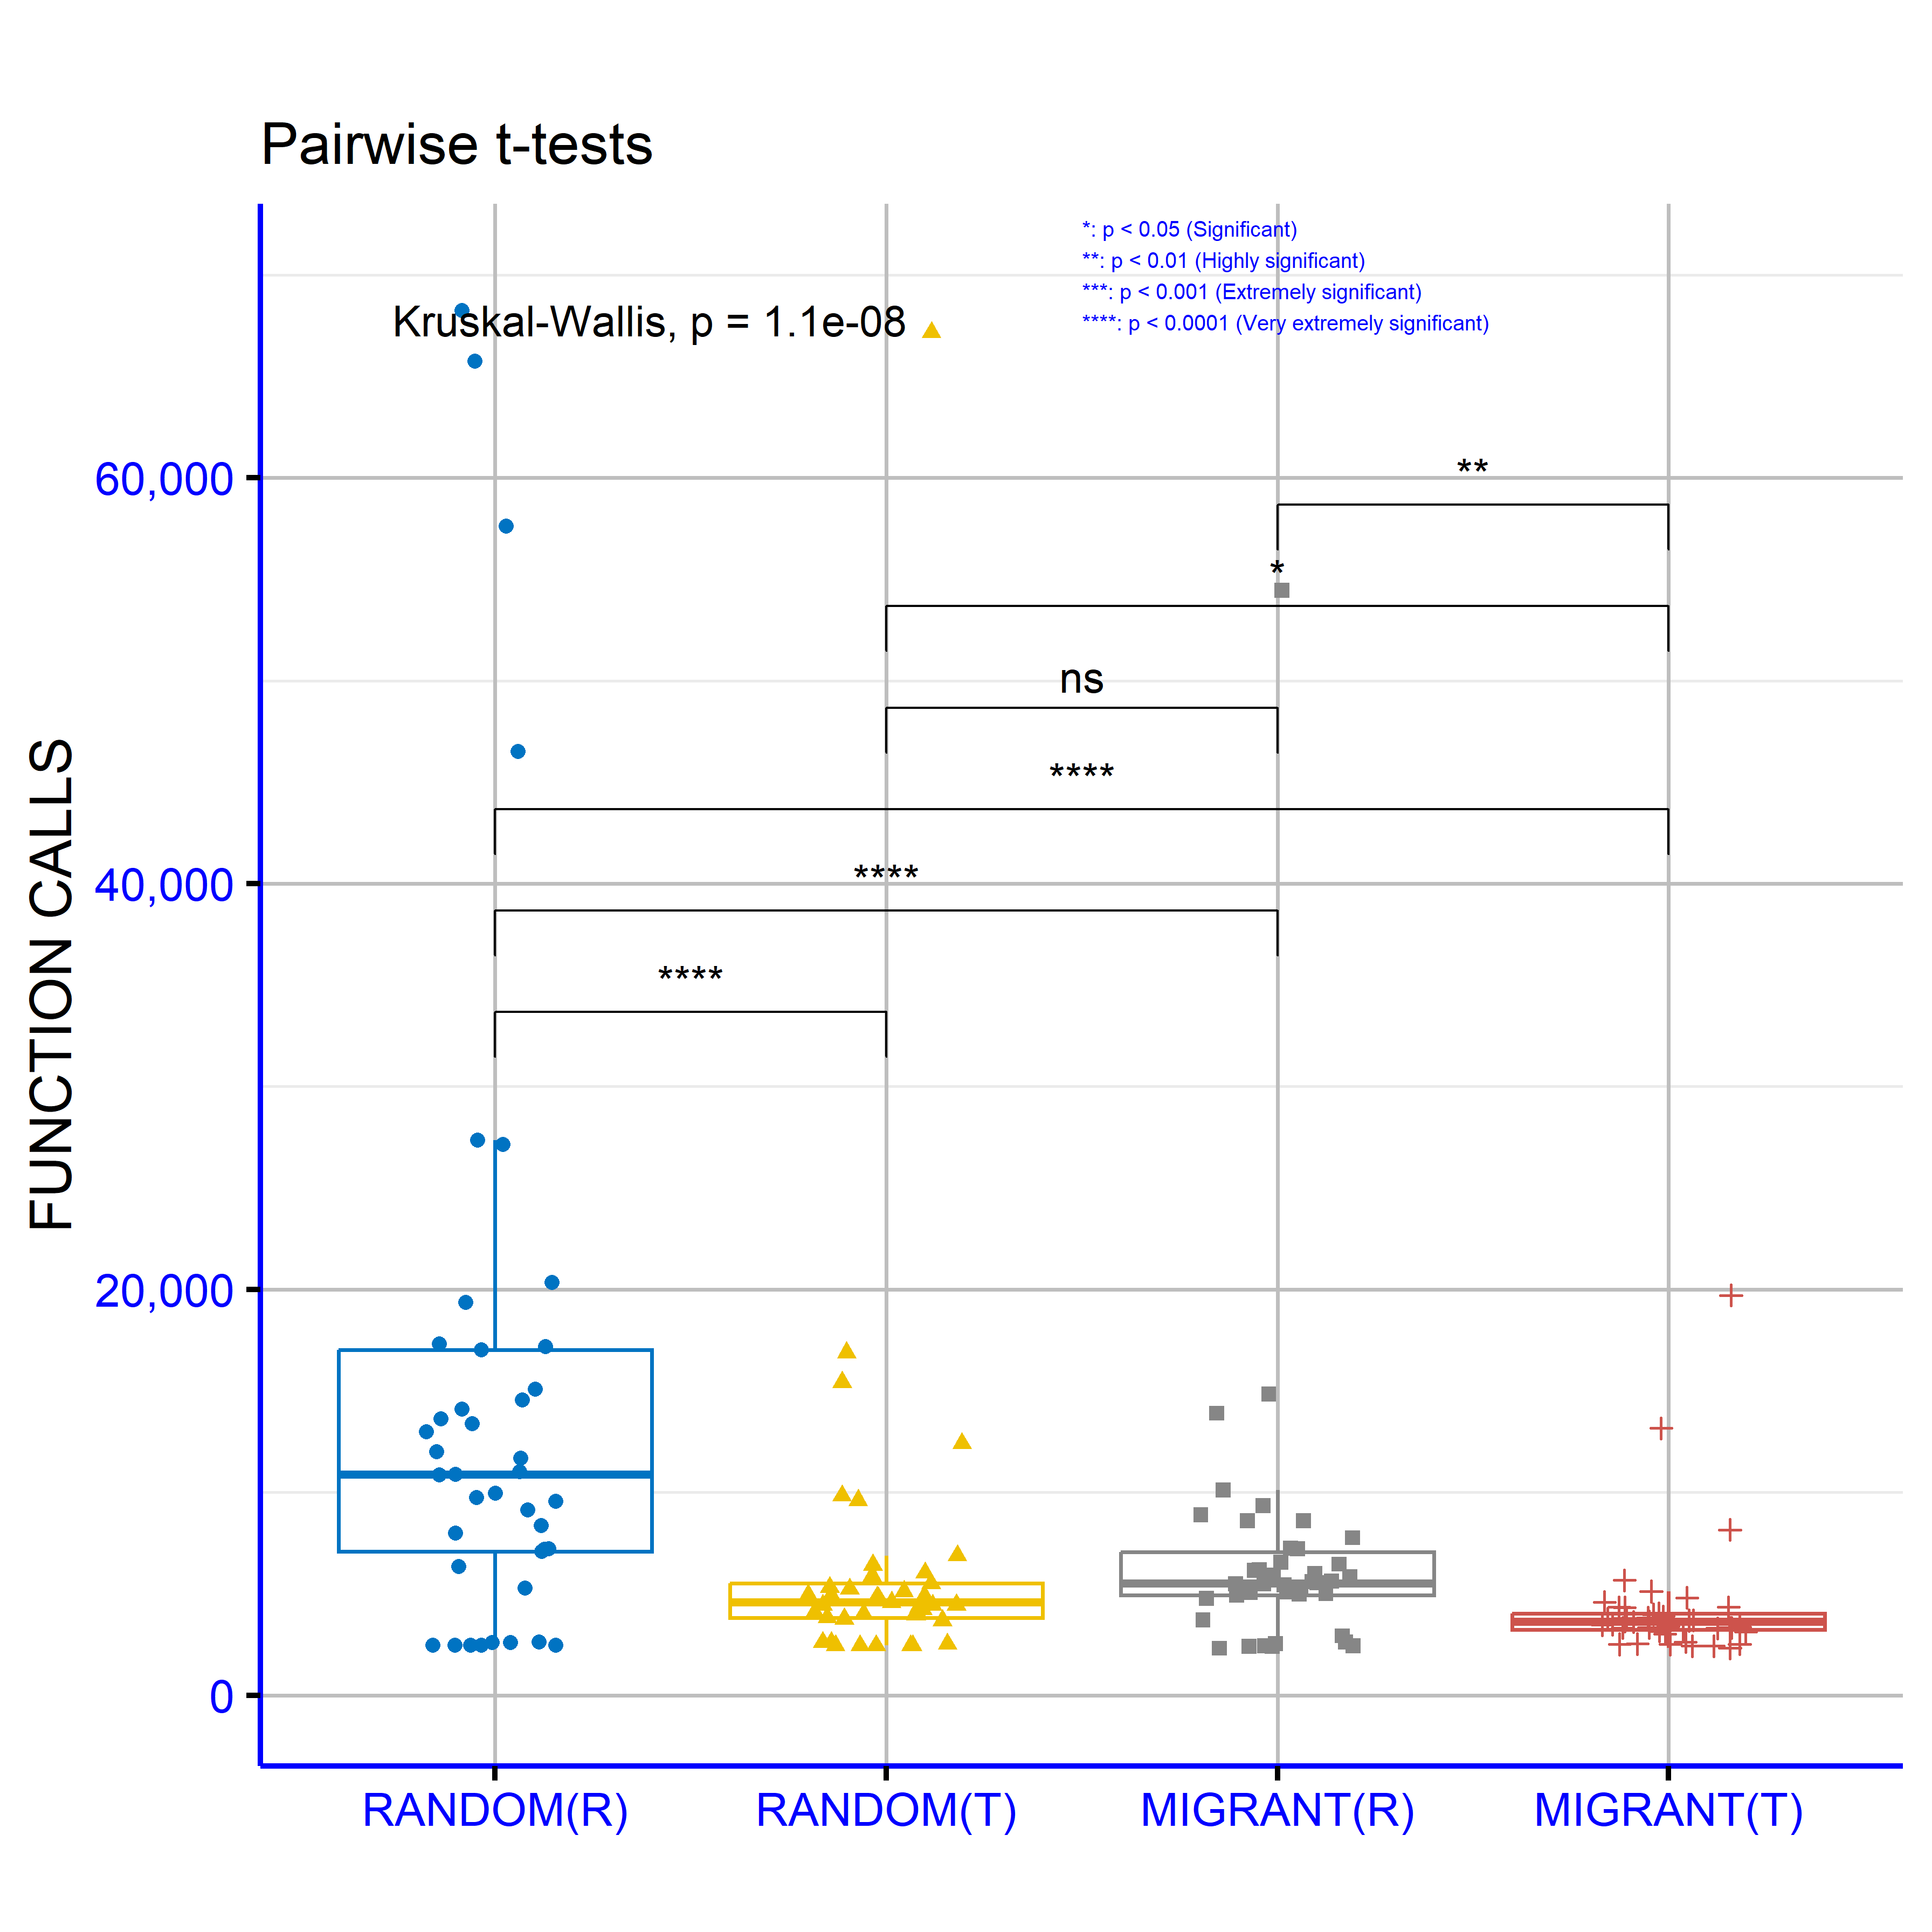
\includegraphics[scale=0.5]{stat2}
\begin{centering}
\caption{Statistical comparison for the used selection methods.\label{fig:statSelection}}
\par\end{centering}
\end{figure}
\par\end{center}

\subsection{The effect of sampling method}

In Table \ref{tab:sampling}, the selection of samples used in the
core formula of differential evolution is conducted through tournament
selection. Four approaches for computing the differential weight are
compared: random weight with uniform sampling (Random(U)), random
weight with k-means sampling (Random(K)), MIGRANT weight with uniform
sampling (Migrant(U)), and MIGRANT weight with k-means sampling (Migrant(K)).
The k-means technique used to locate centers is considered also as
a sampling method here. The method was introduced by James MacQueen\citep{MacQueen}
and it has been considered in a series of research papers \citep{kmeans1,kmeans2}. 

The use of k-means sampling has a decisive impact on reducing the
number of objective function evaluations and improving success rates.
For example, in the Random method, k-means sampling (Random(K)) dramatically
reduces the number of evaluations while significantly increasing success
rates. In function F9 with a dimension of 10, Random(U) requires 71680
evaluations with a success rate of only 3\%, whereas Random(K) reduces
the evaluations to 62309 and boosts the success rate to 97\%. Similar
outcomes are observed in higher dimensions, such as in dimension 20
for the same function, where Random(K) achieves a success rate of
97\% with fewer evaluations (74754) compared to Random(U), which has
a 3\% success rate with 75827 evaluations. A similar impact of k-means
is evident in the MIGRANT method. For instance, in function F12 with
a dimension of 5, MIGRANT(K) reduces the number of evaluations to
2310 while maintaining a notable success rate of 63\%, compared to
MIGRANT(U), which requires 3366 evaluations with a success rate of
90\%. In more demanding functions, such as SCHWEFEL221 with a dimension
of 15, MIGRANT(K) reduces the evaluations to 4134 while maintaining
a success rate of 10\%, whereas MIGRANT(U) requires 5112 evaluations
for the same success rate. The overall effect of k-means sampling
is also reflected in the average results. In the Random method, the
success rate increases from 80\% (Random(U)) to 94\% (Random(K)),
with a significant reduction in evaluations from 503875 to 432601.
Similarly, in the MIGRANT method, MIGRANT(K) achieves an average success
rate of 83\% with only 144826 evaluations, compared to MIGRANT(U),
which has a success rate of 66\% and requires 186307 evaluations.
These findings highlight the critical role of k-means sampling in
reducing computational complexity and enhancing the method’s performance.
The use of k-means provides an effective strategy for boosting success
rates while simultaneously conserving computational resources.

\begin{table}[H]
\caption{Experiments using different sampling techniques\label{tab:sampling}}

\centering{}{\footnotesize{}}%
\begin{tabular}{|c|c|c|c|c|c|}
\hline 
{\footnotesize{}FUNCTION} & {\footnotesize{}DIM} & {\footnotesize{}RANDOM(U)} & {\footnotesize{}RANDOM(K)} & {\footnotesize{}MIGRANT(U)} & {\footnotesize{}MIGRANT(K)}\tabularnewline
\hline 
\hline 
{\footnotesize{}F9} & {\footnotesize{}5} & {\footnotesize{}67178} & {\footnotesize{}42222} & {\footnotesize{}4337(0.23)} & {\footnotesize{}2979}\tabularnewline
\hline 
{\footnotesize{}F9} & {\footnotesize{}10} & {\footnotesize{}71680(0.03)} & {\footnotesize{}62309(0.97)} & {\footnotesize{}8156(0.03)} & {\footnotesize{}6017(0.97)}\tabularnewline
\hline 
{\footnotesize{}F9} & {\footnotesize{}15} & {\footnotesize{}75608(0.03)} & {\footnotesize{}71210} & {\footnotesize{}13156(0.03)} & {\footnotesize{}7990}\tabularnewline
\hline 
{\footnotesize{}F9} & {\footnotesize{}20} & {\footnotesize{}75827(0.03)} & {\footnotesize{}74754} & {\footnotesize{}19711(0.03)} & {\footnotesize{}9592}\tabularnewline
\hline 
{\footnotesize{}F12} & {\footnotesize{}5} & {\footnotesize{}4085} & {\footnotesize{}2745(0.97)} & {\footnotesize{}3366(0.90)} & {\footnotesize{}2310(0.63)}\tabularnewline
\hline 
{\footnotesize{}F12} & {\footnotesize{}10} & {\footnotesize{}4113} & {\footnotesize{}3599} & {\footnotesize{}3135} & {\footnotesize{}2727(0.93)}\tabularnewline
\hline 
{\footnotesize{}F12} & {\footnotesize{}15} & {\footnotesize{}4367} & {\footnotesize{}4060} & {\footnotesize{}3246(0.97)} & {\footnotesize{}3033}\tabularnewline
\hline 
{\footnotesize{}F12} & {\footnotesize{}20} & {\footnotesize{}4916} & {\footnotesize{}4700} & {\footnotesize{}3317(0.90)} & {\footnotesize{}3267}\tabularnewline
\hline 
{\footnotesize{}F13} & {\footnotesize{}5} & {\footnotesize{}4442(0.13)} & {\footnotesize{}2565} & {\footnotesize{}3023(0.03)} & {\footnotesize{}1995}\tabularnewline
\hline 
{\footnotesize{}F13} & {\footnotesize{}10} & {\footnotesize{}9837(0.03)} & {\footnotesize{}6744} & {\footnotesize{}3714(0.03)} & {\footnotesize{}3003}\tabularnewline
\hline 
{\footnotesize{}F13} & {\footnotesize{}15} & {\footnotesize{}6425(0.03)} & {\footnotesize{}5711} & {\footnotesize{}3823(0.03)} & {\footnotesize{}3459}\tabularnewline
\hline 
{\footnotesize{}F13} & {\footnotesize{}20} & {\footnotesize{}5324(0.07)} & {\footnotesize{}5028} & {\footnotesize{}3882(0.10)} & {\footnotesize{}3532}\tabularnewline
\hline 
{\footnotesize{}F14} & {\footnotesize{}5} & {\footnotesize{}3685} & {\footnotesize{}2351} & {\footnotesize{}3162} & {\footnotesize{}2086}\tabularnewline
\hline 
{\footnotesize{}F14} & {\footnotesize{}10} & {\footnotesize{}3824} & {\footnotesize{}3276} & {\footnotesize{}3319} & {\footnotesize{}2858}\tabularnewline
\hline 
{\footnotesize{}F14} & {\footnotesize{}15} & {\footnotesize{}4774(0.80)} & {\footnotesize{}3981(0.37)} & {\footnotesize{}3646(0.47)} & {\footnotesize{}3190(0.10)}\tabularnewline
\hline 
{\footnotesize{}F14} & {\footnotesize{}20} & {\footnotesize{}4438} & {\footnotesize{}4536(0.97)} & {\footnotesize{}3607(0.93)} & {\footnotesize{}3539(0.47)}\tabularnewline
\hline 
{\footnotesize{}F15} & {\footnotesize{}5} & {\footnotesize{}4806(0.50)} & {\footnotesize{}3015(0.53)} & {\footnotesize{}3304(0.20)} & {\footnotesize{}2133(0.20)}\tabularnewline
\hline 
{\footnotesize{}F15} & {\footnotesize{}10} & {\footnotesize{}4837(0.90)} & {\footnotesize{}4161(0.87)} & {\footnotesize{}3683(0.53)} & {\footnotesize{}3149(0.70)}\tabularnewline
\hline 
{\footnotesize{}F15} & {\footnotesize{}15} & {\footnotesize{}4933(0.80)} & {\footnotesize{}4664(0.90)} & {\footnotesize{}3799(0.60)} & {\footnotesize{}3549(0.63)}\tabularnewline
\hline 
{\footnotesize{}F15} & {\footnotesize{}20} & {\footnotesize{}5117} & {\footnotesize{}4914} & {\footnotesize{}3773(0.60)} & {\footnotesize{}3691(0.63)}\tabularnewline
\hline 
{\footnotesize{}F18} & {\footnotesize{}5} & {\footnotesize{}2446} & {\footnotesize{}1612} & {\footnotesize{}2425} & {\footnotesize{}1599}\tabularnewline
\hline 
{\footnotesize{}F18} & {\footnotesize{}10} & {\footnotesize{}2447} & {\footnotesize{}2112} & {\footnotesize{}2325} & {\footnotesize{}2093}\tabularnewline
\hline 
{\footnotesize{}F18} & {\footnotesize{}15} & {\footnotesize{}2450} & {\footnotesize{}2293} & {\footnotesize{}2422} & {\footnotesize{}2274}\tabularnewline
\hline 
{\footnotesize{}F18} & {\footnotesize{}20} & {\footnotesize{}2445} & {\footnotesize{}2376} & {\footnotesize{}2511} & {\footnotesize{}2357}\tabularnewline
\hline 
{\footnotesize{}F19} & {\footnotesize{}5} & {\footnotesize{}2602} & {\footnotesize{}1627} & {\footnotesize{}2502} & {\footnotesize{}1615}\tabularnewline
\hline 
{\footnotesize{}F19} & {\footnotesize{}10} & {\footnotesize{}2447} & {\footnotesize{}2128} & {\footnotesize{}2524} & {\footnotesize{}2107}\tabularnewline
\hline 
{\footnotesize{}F19} & {\footnotesize{}15} & {\footnotesize{}2529} & {\footnotesize{}2312} & {\footnotesize{}2626} & {\footnotesize{}2293}\tabularnewline
\hline 
{\footnotesize{}F19} & {\footnotesize{}20} & {\footnotesize{}2612} & {\footnotesize{}2394} & {\footnotesize{}2533} & {\footnotesize{}2371}\tabularnewline
\hline 
{\footnotesize{}TEST2N} & {\footnotesize{}5} & {\footnotesize{}4448} & {\footnotesize{}2972} & {\footnotesize{}3494(0.97)} & {\footnotesize{}2309}\tabularnewline
\hline 
{\footnotesize{}TEST2N} & {\footnotesize{}10} & {\footnotesize{}6881} & {\footnotesize{}5676} & {\footnotesize{}3980(0.50)} & {\footnotesize{}3374(0.80)}\tabularnewline
\hline 
{\footnotesize{}TEST2N} & {\footnotesize{}15} & {\footnotesize{}9605(0.97)} & {\footnotesize{}8999} & {\footnotesize{}4330(0.17)} & {\footnotesize{}3944(0.20)}\tabularnewline
\hline 
{\footnotesize{}TEST2N} & {\footnotesize{}20} & {\footnotesize{}12407(0.93)} & {\footnotesize{}12059(0.97)} & {\footnotesize{}4595(0.10)} & {\footnotesize{}4351(0.13)}\tabularnewline
\hline 
{\footnotesize{}ELP} & {\footnotesize{}5} & {\footnotesize{}3961} & {\footnotesize{}2600} & {\footnotesize{}3324} & {\footnotesize{}2096}\tabularnewline
\hline 
{\footnotesize{}ELP} & {\footnotesize{}10} & {\footnotesize{}4795} & {\footnotesize{}4002} & {\footnotesize{}3702} & {\footnotesize{}3079}\tabularnewline
\hline 
{\footnotesize{}ELP} & {\footnotesize{}15} & {\footnotesize{}5511} & {\footnotesize{}4884} & {\footnotesize{}4026} & {\footnotesize{}3622}\tabularnewline
\hline 
{\footnotesize{}ELP} & {\footnotesize{}20} & {\footnotesize{}5891} & {\footnotesize{}5569} & {\footnotesize{}4336} & {\footnotesize{}4041}\tabularnewline
\hline 
{\footnotesize{}SCHWEFEL221} & {\footnotesize{}5} & {\footnotesize{}3767} & {\footnotesize{}2421} & {\footnotesize{}3457} & {\footnotesize{}2316}\tabularnewline
\hline 
{\footnotesize{}SCHWEFEL221} & {\footnotesize{}10} & {\footnotesize{}4223} & {\footnotesize{}3545} & {\footnotesize{}3395} & {\footnotesize{}2870}\tabularnewline
\hline 
{\footnotesize{}SCHWEFEL221} & {\footnotesize{}15} & {\footnotesize{}16887(0.23)} & {\footnotesize{}14874(0.03)} & {\footnotesize{}5112(0.03)} & {\footnotesize{}4134(0.10)}\tabularnewline
\hline 
{\footnotesize{}SCHWEFEL221} & {\footnotesize{}20} & {\footnotesize{}15425(0.70)} & {\footnotesize{}15312(0.47)} & {\footnotesize{}5667(0.13)} & {\footnotesize{}5401(0.03)}\tabularnewline
\hline 
{\footnotesize{}SINU} & {\footnotesize{}5} & {\footnotesize{}4013} & {\footnotesize{}2626} & {\footnotesize{}3326(0.77)} & {\footnotesize{}2273(0.73)}\tabularnewline
\hline 
{\footnotesize{}SINU} & {\footnotesize{}10} & {\footnotesize{}4588} & {\footnotesize{}3849} & {\footnotesize{}3648(0.93)} & {\footnotesize{}3058}\tabularnewline
\hline 
{\footnotesize{}SINU} & {\footnotesize{}15} & {\footnotesize{}5240} & {\footnotesize{}4605} & {\footnotesize{}4051(0.87)} & {\footnotesize{}3489}\tabularnewline
\hline 
{\footnotesize{}SINU} & {\footnotesize{}20} & {\footnotesize{}6039} & {\footnotesize{}5209} & {\footnotesize{}4807(0.70)} & {\footnotesize{}3661}\tabularnewline
\hline 
\textbf{\footnotesize{}AVERAGE} &  & \textbf{\footnotesize{}503875(0.80)} & \textbf{\footnotesize{}432601(0.94)} & \textbf{\footnotesize{}186307(0.66)} & \textbf{\footnotesize{}144826(0.83)}\tabularnewline
\hline 
\end{tabular}{\footnotesize\par}
\end{table}

In figure \ref{fig:statSampling}, the general analysis yielded a
p-value of 1e-08. This value is extremely small and significantly
lower than the commonly used significance level (p=0.05). The comparison
between RANDOM(U) and RANDOM(K) produced a p-value of 3e-09. This
exceptionally low value indicates that the two approaches differ significantly
in their results. These differences reflect substantial variations
in performance or behavior. The analysis of RANDOM(U) compared to
MIGRANT(U) resulted in a p-value of 1e-04. Although larger than the
previous values, this p-value remains sufficiently low to indicate
statistically significant differences. This suggests that the two
approaches exhibit distinct performance characteristics that cannot
be ignored. The comparison between RANDOM(U) and MIGRANT(K) yielded
a p-value of 1.6e-06, further supporting the presence of notable differences
between these two approaches. Conversely, the p-value for the comparison
between RANDOM(K) and MIGRANT(U) was 0.056, which exceeds the conventional
significance threshold. This indicates that, in this case, there is
insufficient evidence to conclude statistically significant differences
between these two approaches. The comparison between RANDOM(K) and
MIGRANT(K) produced a p-value of 0.016, which is lower than the significance
threshold (p=0.05). This demonstrates that the two approaches exhibit
some statistically significant differences in their outcomes, albeit
less pronounced than in earlier comparisons. Finally, the analysis
between MIGRANT(U) and MIGRANT(K) yielded two p-values, 3e-09 and
0.00041, both of which are far below the significance level. This
highlights clear and strong differences between these two variations
of the MIGRANT approach, suggesting that the choice of the appropriate
approach can significantly impact performance. In summary, the exceptionally
low p-values observed in most comparisons indicate the presence of
clear differences among the approaches examined. An exception is the
comparison between RANDOM(K) and MIGRANT(U), where no significant
difference was recorded. These findings underscore the importance
of selecting the appropriate method, taking into account the specific
characteristics of each problem and the potential to optimize performance
through careful parameterization.

\begin{figure}[H]
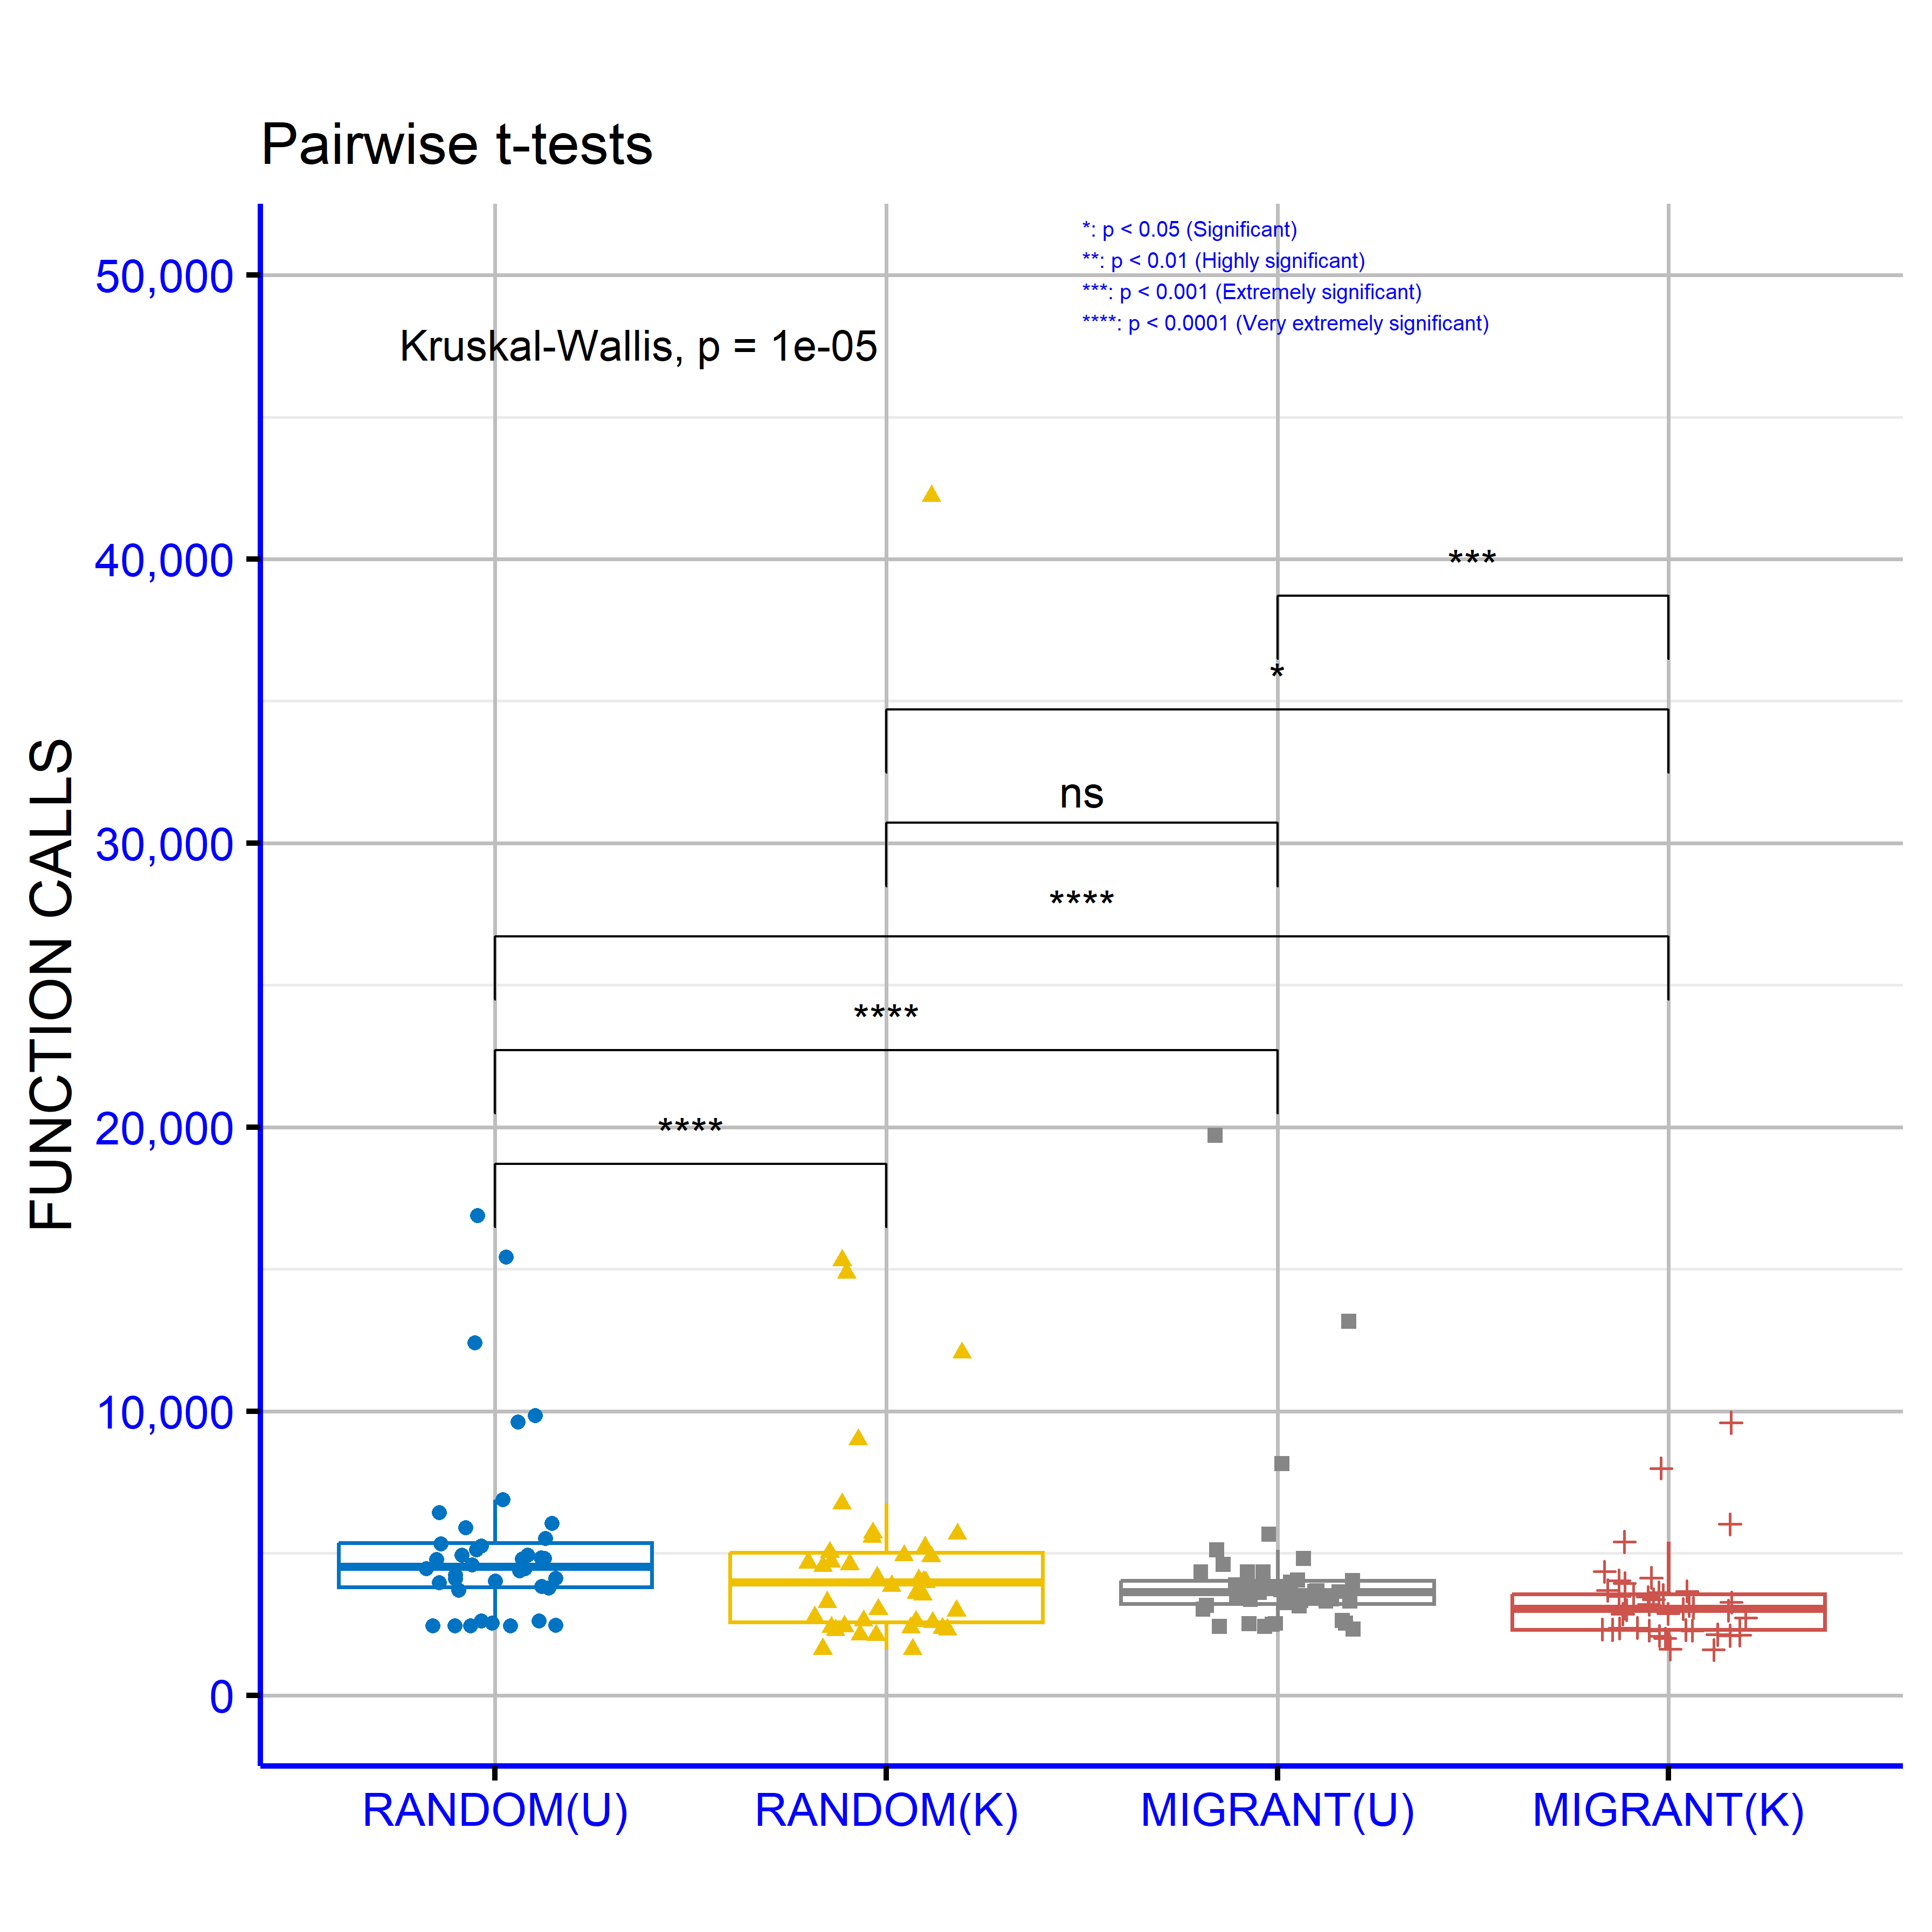
\includegraphics[scale=0.5]{stat3}
\begin{centering}
\caption{Statistical comparison for the different sampling techniques.\label{fig:statSampling}}
\par\end{centering}
\end{figure}


\subsection{The effect of local search rate }

Table \ref{tab:lrate}, similarly to the previous tables, presents
the number of objective function evaluations for various test functions
and dimensions using the differential evolution method. In this case,
the initial distribution is based on the k-means technique, sample
selection is performed using tournament selection, and the differential
weight is calculated stochastically. The difference between the columns
lies in the frequency of applying periodic local search, which is
used for selecting the differential weight. The evaluated frequencies
are 0.005 (0.5\%), 0.01 (1\%), 0.02 (2\%), and 0.04 (4\%). The results
indicate that higher periodic local search frequencies lead to an
increased number of objective function evaluations without a commensurate
improvement in success rates. For instance, in function F9 with a
dimension of 10, a frequency of 0.005 requires 48872 evaluations,
while a frequency of 0.04 increases the evaluations to 151795, more
than threefold. However, the success rate remains at 97\% for both
0.01 and 0.04 frequencies, suggesting that higher frequencies do not
significantly enhance performance. Similar trends are observed in
other functions. In function TEST2N with a dimension of 20, a frequency
of 0.005 requires 11297 evaluations for a success rate of 73\%, whereas
a frequency of 0.01 increases evaluations to 12059, improving the
success rate to 97\%. However, a frequency of 0.04 raises the evaluations
to 14491 without further increasing the success rate. In less demanding
functions, such as F12, the impact of periodic local search frequency
is smaller. For instance, in dimension 5, evaluations range from 2665
to 2488 without noticeable changes in results. This overall trend
is reflected in the averages. With a frequency of 0.005, the average
number of evaluations is 335607 with a success rate of 90\%. A frequency
of 0.01 increases evaluations to 432601, with the success rate reaching
94\%. Higher frequencies, 0.02 and 0.04, lead to 496873 and 714296
evaluations, respectively, with success rates marginally rising to
95\% and 96\%. These findings emphasize the importance of selecting
an optimal frequency for applying periodic local search. While higher
frequencies may provide slight improvements in success rates, the
computational cost increases disproportionately. Lower frequencies,
such as 0.005 or 0.01, appear to offer the best balance between efficiency
and accuracy.

\begin{table}[H]
\caption{Experiments using different values for the local search rate.\label{tab:lrate}}

\centering{}{\footnotesize{}}%
\begin{tabular}{|c|c|c|c|c|c|}
\hline 
{\footnotesize{}FUNCTION} & {\footnotesize{}DIM} & {\footnotesize{}RANDOM(0.005)} & {\footnotesize{}RANDOM(0.01)} & {\footnotesize{}RANDOM(0.02)} & {\footnotesize{}RANDOM(0.04)}\tabularnewline
\hline 
\hline 
{\footnotesize{}F9} & {\footnotesize{}5} & {\footnotesize{}31745} & {\footnotesize{}42222} & {\footnotesize{}50265} & {\footnotesize{}67467}\tabularnewline
\hline 
{\footnotesize{}F9} & {\footnotesize{}10} & {\footnotesize{}48872} & {\footnotesize{}62309(0.97)} & {\footnotesize{}92313} & {\footnotesize{}151795}\tabularnewline
\hline 
{\footnotesize{}F9} & {\footnotesize{}15} & {\footnotesize{}53490} & {\footnotesize{}71210} & {\footnotesize{}102089} & {\footnotesize{}168521}\tabularnewline
\hline 
{\footnotesize{}F9} & {\footnotesize{}20} & {\footnotesize{}55924} & {\footnotesize{}74754} & {\footnotesize{}109991} & {\footnotesize{}179798}\tabularnewline
\hline 
{\footnotesize{}F12} & {\footnotesize{}5} & {\footnotesize{}2665} & {\footnotesize{}2745(0.97)} & {\footnotesize{}2641} & {\footnotesize{}2488}\tabularnewline
\hline 
{\footnotesize{}F12} & {\footnotesize{}10} & {\footnotesize{}3460} & {\footnotesize{}3599} & {\footnotesize{}3749} & {\footnotesize{}3916}\tabularnewline
\hline 
{\footnotesize{}F12} & {\footnotesize{}15} & {\footnotesize{}4043} & {\footnotesize{}4060} & {\footnotesize{}4275} & {\footnotesize{}4630}\tabularnewline
\hline 
{\footnotesize{}F12} & {\footnotesize{}20} & {\footnotesize{}4581} & {\footnotesize{}4700} & {\footnotesize{}4877} & {\footnotesize{}5118}\tabularnewline
\hline 
{\footnotesize{}F13} & {\footnotesize{}5} & {\footnotesize{}2395} & {\footnotesize{}2565} & {\footnotesize{}2873} & {\footnotesize{}3513}\tabularnewline
\hline 
{\footnotesize{}F13} & {\footnotesize{}10} & {\footnotesize{}6635} & {\footnotesize{}6744} & {\footnotesize{}6975} & {\footnotesize{}7439}\tabularnewline
\hline 
{\footnotesize{}F13} & {\footnotesize{}15} & {\footnotesize{}5793} & {\footnotesize{}5711} & {\footnotesize{}5655} & {\footnotesize{}6251}\tabularnewline
\hline 
{\footnotesize{}F13} & {\footnotesize{}20} & {\footnotesize{}5246} & {\footnotesize{}5028} & {\footnotesize{}5104} & {\footnotesize{}6080}\tabularnewline
\hline 
{\footnotesize{}F14} & {\footnotesize{}5} & {\footnotesize{}2139} & {\footnotesize{}2351} & {\footnotesize{}2803} & {\footnotesize{}3459}\tabularnewline
\hline 
{\footnotesize{}F14} & {\footnotesize{}10} & {\footnotesize{}2939} & {\footnotesize{}3276} & {\footnotesize{}3817} & {\footnotesize{}4662}\tabularnewline
\hline 
{\footnotesize{}F14} & {\footnotesize{}15} & {\footnotesize{}3481(0.20)} & {\footnotesize{}3981(0.37)} & {\footnotesize{}5168(0.63)} & {\footnotesize{}6363(0.87)}\tabularnewline
\hline 
{\footnotesize{}F14} & {\footnotesize{}20} & {\footnotesize{}4010(0.90)} & {\footnotesize{}4536(0.97)} & {\footnotesize{}5297(0.93)} & {\footnotesize{}6597}\tabularnewline
\hline 
{\footnotesize{}F15} & {\footnotesize{}5} & {\footnotesize{}2571(0.27)} & {\footnotesize{}3015(0.53)} & {\footnotesize{}3639(0.73)} & {\footnotesize{}4574(0.73)}\tabularnewline
\hline 
{\footnotesize{}F15} & {\footnotesize{}10} & {\footnotesize{}3516(0.70)} & {\footnotesize{}4161(0.87)} & {\footnotesize{}4943(0.93)} & {\footnotesize{}6409}\tabularnewline
\hline 
{\footnotesize{}F15} & {\footnotesize{}15} & {\footnotesize{}3887(0.43)} & {\footnotesize{}4664(0.90)} & {\footnotesize{}5933(0.97)} & {\footnotesize{}7581}\tabularnewline
\hline 
{\footnotesize{}F15} & {\footnotesize{}20} & {\footnotesize{}4211} & {\footnotesize{}4914} & {\footnotesize{}5870} & {\footnotesize{}7560}\tabularnewline
\hline 
{\footnotesize{}F18} & {\footnotesize{}5} & {\footnotesize{}1597} & {\footnotesize{}1612} & {\footnotesize{}1643} & {\footnotesize{}1703}\tabularnewline
\hline 
{\footnotesize{}F18} & {\footnotesize{}10} & {\footnotesize{}2093} & {\footnotesize{}2112} & {\footnotesize{}2152} & {\footnotesize{}2228}\tabularnewline
\hline 
{\footnotesize{}F18} & {\footnotesize{}15} & {\footnotesize{}2273} & {\footnotesize{}2293} & {\footnotesize{}2334} & {\footnotesize{}2416}\tabularnewline
\hline 
{\footnotesize{}F18} & {\footnotesize{}20} & {\footnotesize{}2356} & {\footnotesize{}2376} & {\footnotesize{}2423} & {\footnotesize{}2510}\tabularnewline
\hline 
{\footnotesize{}F19} & {\footnotesize{}5} & {\footnotesize{}1613} & {\footnotesize{}1627} & {\footnotesize{}1660} & {\footnotesize{}1715}\tabularnewline
\hline 
{\footnotesize{}F19} & {\footnotesize{}10} & {\footnotesize{}2109} & {\footnotesize{}2128} & {\footnotesize{}2170} & {\footnotesize{}2243}\tabularnewline
\hline 
{\footnotesize{}F19} & {\footnotesize{}15} & {\footnotesize{}2290} & {\footnotesize{}2312} & {\footnotesize{}2351} & {\footnotesize{}2433}\tabularnewline
\hline 
{\footnotesize{}F19} & {\footnotesize{}20} & {\footnotesize{}2371} & {\footnotesize{}2394} & {\footnotesize{}2437} & {\footnotesize{}2519}\tabularnewline
\hline 
{\footnotesize{}TEST2N} & {\footnotesize{}5} & {\footnotesize{}2893} & {\footnotesize{}2972} & {\footnotesize{}3060} & {\footnotesize{}3274}\tabularnewline
\hline 
{\footnotesize{}TEST2N} & {\footnotesize{}10} & {\footnotesize{}5608} & {\footnotesize{}5676} & {\footnotesize{}6112} & {\footnotesize{}6832}\tabularnewline
\hline 
{\footnotesize{}TEST2N} & {\footnotesize{}15} & {\footnotesize{}8576(0.90)} & {\footnotesize{}8999} & {\footnotesize{}9279} & {\footnotesize{}10464}\tabularnewline
\hline 
{\footnotesize{}TEST2N} & {\footnotesize{}20} & {\footnotesize{}11297(0.73)} & {\footnotesize{}12059(0.97)} & {\footnotesize{}12908(0.97)} & {\footnotesize{}14491}\tabularnewline
\hline 
{\footnotesize{}ELP} & {\footnotesize{}5} & {\footnotesize{}2645} & {\footnotesize{}2600} & {\footnotesize{}2486} & {\footnotesize{}2486}\tabularnewline
\hline 
{\footnotesize{}ELP} & {\footnotesize{}10} & {\footnotesize{}4295} & {\footnotesize{}4002} & {\footnotesize{}3882} & {\footnotesize{}3890}\tabularnewline
\hline 
{\footnotesize{}ELP} & {\footnotesize{}15} & {\footnotesize{}5206} & {\footnotesize{}4884} & {\footnotesize{}4918} & {\footnotesize{}5004}\tabularnewline
\hline 
{\footnotesize{}ELP} & {\footnotesize{}20} & {\footnotesize{}5965} & {\footnotesize{}5569} & {\footnotesize{}5486} & {\footnotesize{}5944}\tabularnewline
\hline 
{\footnotesize{}SCHWEFEL221} & {\footnotesize{}5} & {\footnotesize{}2616} & {\footnotesize{}2421} & {\footnotesize{}2354} & {\footnotesize{}2233}\tabularnewline
\hline 
{\footnotesize{}SCHWEFEL221} & {\footnotesize{}10} & {\footnotesize{}3596} & {\footnotesize{}3545} & {\footnotesize{}3520} & {\footnotesize{}3630}\tabularnewline
\hline 
{\footnotesize{}SCHWEFEL221} & {\footnotesize{}15} & {\footnotesize{}14182(0.03)} & {\footnotesize{}14874(0.03)} & {\footnotesize{}14716(0.07)} & {\footnotesize{}15641(0.27)}\tabularnewline
\hline 
{\footnotesize{}SCHWEFEL221} & {\footnotesize{}20} & {\footnotesize{}15674(0.53)} & {\footnotesize{}15312(0.47)} & {\footnotesize{}16252(0.53)} & {\footnotesize{}17924(0.57)}\tabularnewline
\hline 
{\footnotesize{}SINU} & {\footnotesize{}5} & {\footnotesize{}2600} & {\footnotesize{}2626} & {\footnotesize{}2775} & {\footnotesize{}2917}\tabularnewline
\hline 
{\footnotesize{}SINU} & {\footnotesize{}10} & {\footnotesize{}3845} & {\footnotesize{}3849} & {\footnotesize{}3912} & {\footnotesize{}4215}\tabularnewline
\hline 
{\footnotesize{}SINU} & {\footnotesize{}15} & {\footnotesize{}4729} & {\footnotesize{}4605} & {\footnotesize{}4674} & {\footnotesize{}5094}\tabularnewline
\hline 
{\footnotesize{}SINU} & {\footnotesize{}20} & {\footnotesize{}5320} & {\footnotesize{}5209} & {\footnotesize{}5357} & {\footnotesize{}5736}\tabularnewline
\hline 
\textbf{\footnotesize{}AVERAGE} &  & \textbf{\footnotesize{}335607(0.90)} & \textbf{\footnotesize{}432601(0.94)} & \textbf{\footnotesize{}496873(0.95)} & \textbf{\footnotesize{}714296(0.96)}\tabularnewline
\hline 
\end{tabular}{\footnotesize\par}
\end{table}

The general analysis for all pairwise comparisons shown in figure
\ref{fig:statLrate} produced a p-value of 0.49. This value is much
higher than the conventional significance threshold (p=0.05), indicating
that the comparisons overall do not exhibit statistically significant
differences. This observation suggests that, when considered collectively,
the differences among the comparisons might result from random factors.
The comparison between the RANDOM(0.005) and RANDOM(0.01) approaches
yielded a p-value of 0.019. This value is below the significance threshold,
indicating statistically significant differences between these two
approaches. These differences are likely attributable to changes in
the frequency of applying periodic local search. The analysis of RANDOM(0.005)
versus RANDOM(0.02) produced a p-value of 0.00046. This very low value
demonstrates clear statistically significant differences between the
two approaches, reflecting substantial performance changes due to
the increased application frequency. The comparison between RANDOM(0.005)
and RANDOM(0.04) yielded a p-value of 8.3e-06, which is extremely
low. This indicates that the two approaches exhibit significantly
different performance, likely due to the very high local search frequency
in RANDOM(0.04). The analysis of RANDOM(0.01) versus RANDOM(0.02)
yielded a p-value of 0.0001. Statistically significant differences
are again evident, suggesting that the increase in frequency markedly
affects the results. The comparison between RANDOM(0.01) and RANDOM(0.04)
produced a p-value of 1.7e-06. This extremely low value confirms the
presence of clear differences in the performance of the two approaches,
due to the further frequency increase. Lastly, the comparison between
RANDOM(0.02) and RANDOM(0.04) yielded a p-value of 3.1e-09. This exceptionally
small value demonstrates that the increasing frequency of local search
continues to significantly influence performance. Overall, the low
p-values in most comparisons suggest that the frequency of periodic
local search application significantly affects the performance of
the approaches. However, the general analysis with p=0.49 indicates
that, in combination, the approaches may not show significant differentiation.
These findings underscore the importance of carefully tuning the frequency
of local search application to achieve an optimal balance between
performance and computational cost.

\begin{figure}[H]
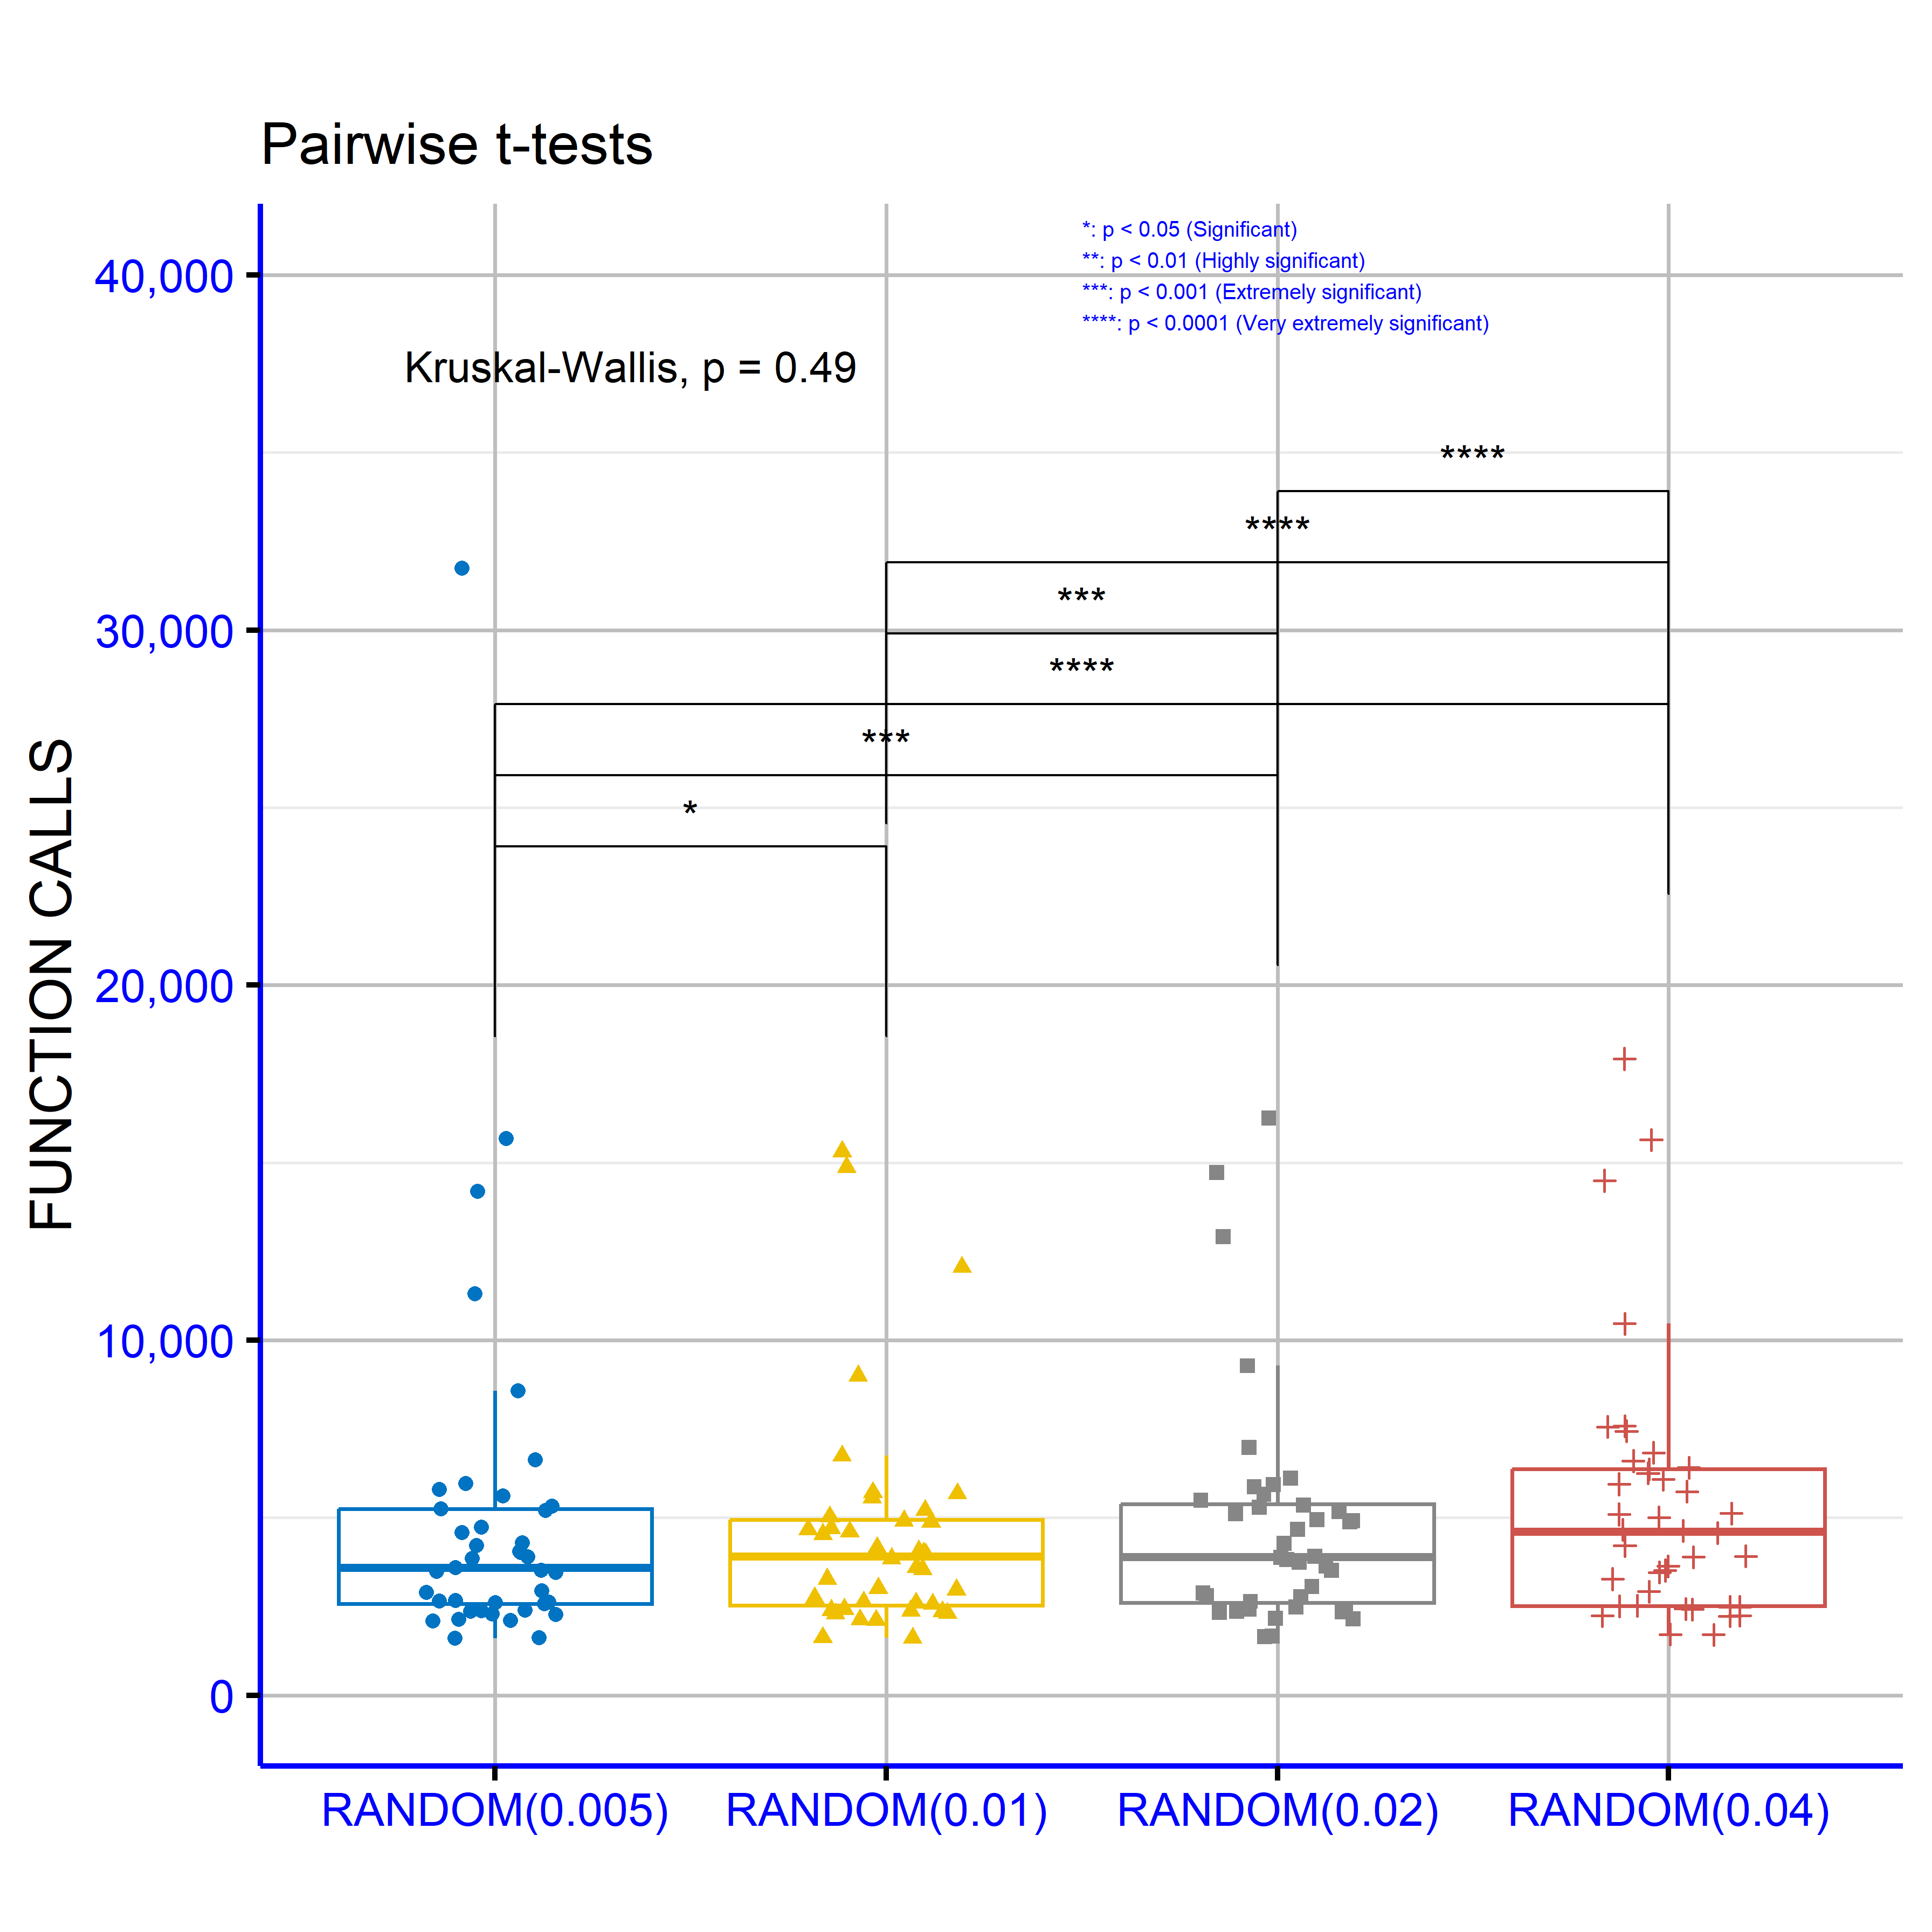
\includegraphics[scale=0.5]{stat4}

\caption{Statistical comparison for the proposed method and different values
of parameter $p_{l}$.\label{fig:statLrate}}

\end{figure}


\subsection{Practical problems}

The proposed method was tested on some problems inspired by real world,
such as the molecular conformation of some atoms or the training of
neural networks.

\subsubsection{Lennard Jones Potential}

The first case of practical function is the energy obtained by the
molecular conformation of N atoms, that interacts using the Lennard-Jones
potential \citep{Jones}. The Lennard-Jones potential (LJ) is arguably
the most widely used pair potential in Molecular Simulation. One of
the most widely used intermolecular potentials in classical many-body
simulations, is the so-called Lennard-Jones potential:
\[
V_{LJ}(r)=4\epsilon\left[\left(\frac{\sigma}{r}\right)^{12}-\left(\frac{\sigma}{r}\right)^{6}\right]
\]

where $\epsilon$ denotes the depth of the attractive well, and the
$\sigma$ interparticle distance where the potential changes sign.
Lennard- Jones-type $r^{-n}~-r^{-m}$ pair potentials were proposed
in 1925 by Jones1 (later Lennard-Jones) to describe the cohesive energy
of crystals of noble gases, such as Argon\citep{key-6}. 

In table \ref{tab:experPotential} the function calls using the proposed
method for this potential are shown. In column NUMBER the results
using the number variant of differential weight are shown, while in
column RANDOM the average function calls obtained by the Random variance
of the differential weight are shown.

\begin{table}[H]
\caption{Experiments for the Lennard - Jones potential using two different
differential weight mechanisms.\label{tab:experPotential}}

\centering{}%
\begin{tabular}{|c|c|c|}
\hline 
ATOMS & NUMBER & RANDOM\tabularnewline
\hline 
\hline 
2 & 2982 & 2844\tabularnewline
\hline 
3 & 3856 & 3673\tabularnewline
\hline 
4 & 5385 & 5183\tabularnewline
\hline 
5 & 8012 & 6920\tabularnewline
\hline 
6 & 12866 & 10995\tabularnewline
\hline 
7 & 21288 & 17577\tabularnewline
\hline 
8 & 35714 & 31866\tabularnewline
\hline 
9 & 57342 & 53424\tabularnewline
\hline 
10 & 89383 & 77893\tabularnewline
\hline 
11 & 113164 & 108395\tabularnewline
\hline 
12 & 144190 & 125621\tabularnewline
\hline 
13 & 146164 & 134219\tabularnewline
\hline 
14 & 171496 & 166035\tabularnewline
\hline 
15 & 195007 & 193038\tabularnewline
\hline 
\textbf{SUM} & \textbf{1006849} & \textbf{937683}\tabularnewline
\hline 
\end{tabular}
\end{table}
Also in Figure \ref{fig:potential} the plot of the function calls
against the number of atoms for the previously used differential weight
mechanisms is shown.

\begin{figure}[H]
\begin{centering}
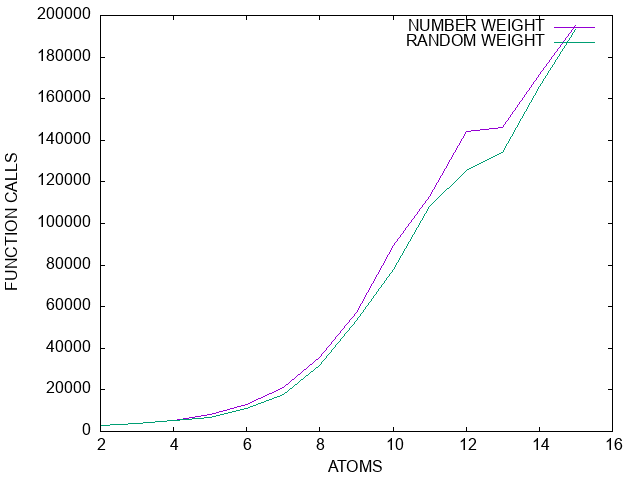
\includegraphics[scale=0.5]{potential_plot}
\par\end{centering}
\caption{Plot of the function calls for the Lennard - Jones potential using
two differential weight mechanisms.\label{fig:potential}}

\end{figure}
As can be seen from the table of results and the relevant graph, the
method that uses the random technique for the differential weight
has slightly better results than the technique that uses a fixed differential
weight. 

\subsubsection{Neural network training}

Another interesting problem where the proposed method can be applied
is the training of artificial neural networks for classification or
regression problems.\textbf{ }Artificial Neural networks (ANNs) \citep{nn1,nn2}
are parametric tools machine learning tools that have been used widely
in a series of real - world problems, such as problems from physics
\citep{nnphysics1,nnphysics2,nnphysics3}, chemistry \citep{nnchem1,nnchem2,nnchem3},
economics \citep{nnecon1,nnecon2,nncecon3}, medicine \citep{nnmed1,nnmed2}
etc. Artificial neural networks are usually expressed as a function
$N(\overrightarrow{x},\overrightarrow{w})$, where the vector $\overrightarrow{x}$
defines the input pattern and the vector $\overrightarrow{w}$ stands
for the weight vector of the neural network (set of parameters). The
training of the neural network is performed with the adjustment of
vector $\overrightarrow{w}$in order to minimize the so - called training
error which is expressed as:

\begin{equation}
E\left(N\left(\overrightarrow{x},\overrightarrow{w}\right)\right)=\sum_{i=1}^{M}\left(N\left(\overrightarrow{x}_{i},\overrightarrow{w}\right)-y_{i}\right)^{2}\label{eq:eq1}
\end{equation}
The set $\left(\overrightarrow{x_{i}},y_{i}\right),\ i=1,...,M$ represents
the train set of the neural network. The value $y_{i}$ stand for
the actual output for pattern $\overrightarrow{x_{i}}$ . 

The proposed method was applied to train a neural network with $H=10$
processing nodes for the following series of classification datasets,
found in the relevant literature \citep{UCL,Keel}:
\begin{enumerate}
\item \textbf{Pima} dataset \citep{pima}, which is used to detect the presence
of the diabetes disease.
\item \textbf{Regions2} dataset, related to the detection hepatitis C \citep{regions}. 
\item \textbf{Wdbc} dataset \citep{wdbc}, a medical related to breast cancer
detection.
\item \textbf{Wine} dataset, used for the detection of quality of wines
\citep{wine1,wine2}.
\item \textbf{Eeg} datasets, a dataset related to EEG measurements \citep{eeg}.
In the conducted experiments the case of Z\_F\_S was used.
\item \textbf{Zoo} dataset \citep{zoo}, used to classify animals.
\end{enumerate}
The experimental results using the proposed method and a series of
differential weight methods are shown in Table \ref{tab:expNeural}.

\begin{table}[H]
\caption{Application of the proposed method with a series of differential weights
on a neural network used for data classification problems. Numbers
in cells represent average classification error as measured on the
test set of the objective problem.\label{tab:expNeural}}

\centering{}%
\begin{tabular}{|c|c|c|c|}
\hline 
DATASET & NUMBER & RANDOM & MIGRANT\tabularnewline
\hline 
\hline 
PIMA & 33.91\% & 33.71\% & 26.99\%\tabularnewline
\hline 
REGIONS2 & 28.98\% & 29.04\% & 28.54\%\tabularnewline
\hline 
WDBC & 8.22\% & 7.32\% & 4.51\%\tabularnewline
\hline 
WINE & 23.22\% & 23.14\% & 9.26\%\tabularnewline
\hline 
Z\_F\_S & 21.39\% & 19.17\% & 8.16\%\tabularnewline
\hline 
ZOO & 6.77\% & 6.70\% & 3.13\%\tabularnewline
\hline 
\textbf{AVERAGE} & \textbf{20.42\%} & \textbf{19.76\%} & \textbf{13.43\%}\tabularnewline
\hline 
\end{tabular}
\end{table}
As it can be deduced from this table, the method MIGRANT proved to
be more effective in terms of classification error from the other
methods.

\section{Discussion}

The experimental results presented in the above tables and figures
provide valuable insights into the performance and characteristics
of the proposed methods. Below, we analyze the findings in detail,
highlighting key conclusions.

\textbf{1. Statistical Comparisons and General Performance}

Figure 1 demonstrates a statistical comparison of the proposed method's
variants applied to a series of objective problems. The extremely
low p-values across all comparisons indicate significant differences
among the methods, emphasizing their unique characteristics. These
differences reflect variations in their ability to reduce the number
of objective function evaluations and achieve high success rates.
The results underscore the importance of selecting the most suitable
variant depending on the specific requirements of the optimization
problem. 

Moreover in table 2, the proposed method achieved significantly fewer
objective function calls compared to the other methods, demonstrating
superior efficiency and reduced computational cost. These differences
confirmed by the Friedman test, and became even more pronounced in
high-dimensional or complex problems. This highlights the proposed
method as a reliable choice for various optimization tasks.

\textbf{2. Selection Mechanisms}

The impact of selection methods is evident in Table 3 and Figure 2.
The experimental results comparing random selection and tournament
selection reveal significant differences, as indicated by the low
p-values. Tournament selection consistently outperformed random selection
in most cases, suggesting that its systematic approach to choosing
individuals based on performance provides a distinct advantage. 

\textbf{3. Sampling Techniques}

Figure 3 highlights the comparative analysis of different sampling
techniques. Although detailed findings are not explicitly stated,
the results reaffirm the importance of carefully selecting sampling
methods to maximize efficiency and ensure robust optimization. Future
research could delve deeper into exploring these techniques interplay
with specific problem domains. 

\textbf{4. Local Search Rate }

Table 5 and Figure 4 reveal the influence of local search rate and
the pi parameter on performance. The experiments indicate that the
optimal frequency for periodic local search lies between 0.005 and
0.01, striking a balance between accuracy and computational cost.
Higher frequencies marginally improve hit rates but at a disproportionate
computational expense. Similarly, tuning the pi parameter is critical
to maintaining this balance. These findings highlight the significance
of methodical parameterization in achieving optimal results. 

\textbf{5. Lennard-Jones potential}

Table 6 showcases the experiments conducted using two differential
weight mechanisms for the Lennard-Jones potential. The method employing
a random differential weight technique consistently yielded better
results than the fixed differential weight approach. This suggests
that introducing variability in the weight mechanism can enhance adaptability
and performance in complex optimization landscapes. 

\textbf{6. Application to Neural Network Classification}

Table 7 reports the application of the proposed method with varying
differential weights for data classification in neural networks. The
MIGRANT method emerged as the most efficient, achieving lower classification
errors compared to alternative approaches. These findings indicate
that the proposed method's adaptability and parameter tuning capabilities
make it particularly effective in high-dimensional, real-world problems
such as data classification. 

The results emphasize the importance of tailoring the optimization
method to the problem’s requirements, leveraging statistical analyses
to guide decision-making. Future work could focus on exploring their
scalability to larger datasets and more complex problems. Expanding
the application scope to other domains, such as dynamic optimization
or multi-objective problems, could further validate the proposed method's
robustness and versatility. 

In conclusion, the analysis highlights the strength of the proposed
methods in adapting to various challenges while providing a framework
for further exploration and refinement.

\section{Conclusions\label{sec:Conclusions}}

This study focuses on large-scale optimization through a modified
version of the Differential Evolution algorithm. The introduced modifications
aim to enhance efficiency and reliability in high-dimensional problems.
Key elements of the new approach include the Migrant differential
weight mechanism and the use of k-means sampling to optimize sample
selection. Experimental results demonstrated that the proposed method
significantly reduces the number of objective function evaluations,
particularly for high-dimensional problems. Variants of the differential
weight mechanism, such as Migrant, offer competitive advantages with
higher success rates and reduced computational cost compared to traditional
approaches. Additionally, the use of k-means sampling contributes
to reduced complexity and improves the algorithm’s performance. In
experimental tests, such as neural network training and molecular
conformation optimization using the Lennard-Jones potential, the algorithm
showcased exceptional capability in finding optimal solutions. However,
the algorithm’s performance is sensitive to parameter tuning, such
as the local search rate. It was observed that higher local search
frequencies can substantially increase computational costs without
a corresponding improvement in success rates, highlighting the need
for a careful balance between accuracy and efficiency. 

Future research could focus on several directions to further enhance
the method. An important aspect is the development of adaptive parameter
tuning strategies that dynamically adjust to the nature of the problem.
Moreover, applying the algorithm in distributed computing environments
could increase its scalability and speed, making it suitable for real-time
problems. Additionally, integrating the algorithm into more complex
dynamic systems, such as economic forecasting problems or simulations
of physical phenomena, represents a promising avenue. Finally, evaluating
the algorithm's performance in large-scale machine learning applications,
such as training deep neural networks, may reveal new capabilities
and applications. Overall, the study highlights the potential of the
proposed approach and emphasizes the importance of continued research
to develop even more efficient and versatile optimization algorithms.

\authorcontributions{G.K., V.C. and I.G.T. conceived of the idea and the methodology,
and G.K. and V.C. implemented the corresponding software. G.K. conducted
the experiments, employing objective functions as test cases, and
provided the comparative experiments. I.G.T. performed the necessary
statistical tests. All authors have read and agreed to the published
version of the manuscript.}

\funding{This research received no external funding.}

\institutionalreview{Not Applicable.}

\informedconsent{Not applicable.}

\acknowledgments{This research has been financed by the European Union: Next Generation
EU through the Program Greece 2.0 National Recovery and Resilience
Plan, under the call RESEARCH--CREATE--INNOVATE, project name “iCREW:
Intelligent small craft simulator for advanced crew training using
Virtual Reality techniques” (project code: TAEDK-06195).}

\conflictsofinterest{The authors declare no conflicts of interest.}

\appendixtitles{no}

\begin{adjustwidth}{-\extralength}{0cm}{}

\begin{thebibliography}{999}
\bibitem{go_math1}Carrizosa, E., Molero-Río, C., \& Romero Morales,
D. (2021). Mathematical optimization in classification and regression
trees. Top, 29(1), 5-33.

\bibitem{go_math3}Legat, B., Dowson, O., Garcia, J. D., \& Lubin,
M. (2022). MathOptInterface: a data structure for mathematical optimization
problems. INFORMS Journal on Computing, 34(2), 672-689.

\bibitem{go_physics2}Su, H., Zhao, D., Heidari, A. A., Liu, L., Zhang,
X., Mafarja, M., \& Chen, H. (2023). RIME: A physics-based optimization.
Neurocomputing, 532, 183-214.

\bibitem{go_physics3}Stilck França, D., \& Garcia-Patron, R. (2021).
Limitations of optimization algorithms on noisy quantum devices. Nature
Physics, 17(11), 1221-1227.

\bibitem{go_chem1}Zhang, J., \& Glezakou, V. A. (2021). Global optimization
of chemical cluster structures: Methods, applications, and challenges.
International Journal of Quantum Chemistry, 121(7), e26553.

\bibitem{go_chem2}Hu, Y., Zang, Z., Chen, D., Ma, X., Liang, Y.,
You, W., \& Zhang, Z. (2022). Optimization and evaluation of SO2 emissions
based on WRF-Chem and 3DVAR data assimilation. Remote Sensing, 14(1),
220.

\bibitem{go_med2}Kaur, P., \& Singh, R. K. (2023). A review on optimization
techniques for medical image analysis. Concurrency and Computation:
Practice and Experience, 35(1), e7443.

\bibitem{medicine}Houssein, E. H., Hosney, M. E., Mohamed, W. M.,
Ali, A. A., \& Younis, E. M. (2023). Fuzzy-based hunger games search
algorithm for global optimization and feature selection using medical
data. Neural Computing and Applications, 35(7), 5251-5275.

\bibitem{go_bio1}Wang, L., Cao, Q., Zhang, Z., Mirjalili, S., \&
Zhao, W. (2022). Artificial rabbits optimization: A new bio-inspired
meta-heuristic algorithm for solving engineering optimization problems.
Engineering Applications of Artificial Intelligence, 114, 105082.

\bibitem{go_bio2}Hesami, M., \& Jones, A. M. P. (2020). Application
of artificial intelligence models and optimization algorithms in plant
cell and tissue culture. Applied Microbiology and Biotechnology, 104(22),
9449-9485.

\bibitem{go_agri1}Filip, M., Zoubek, T., Bumbalek, R., Cerny, P.,
Batista, C. E., Olsan, P., ... \& Findura, P. (2020). Advanced computational
methods for agriculture machinery movement optimization with applications
in sugarcane production. Agriculture, 10(10), 434.

\bibitem{go_agri2}Akintuyi, O. B. (2024). Adaptive AI in precision
agriculture: a review: investigating the use of self-learning algorithms
in optimizing farm operations based on real-time data. Research Journal
of Multidisciplinary Studies, 7(02), 016-030.

\bibitem{go_econ1}Wang, Y., Ma, Y., Song, F., Ma, Y., Qi, C., Huang,
F., ... \& Zhang, F. (2020). Economic and efficient multi-objective
operation optimization of integrated energy system considering electro-thermal
demand response. Energy, 205, 118022.

\bibitem{go_econ2}Alirahmi, S. M., Mousavi, S. B., Razmi, A. R.,
\& Ahmadi, P. (2021). A comprehensive techno-economic analysis and
multi-criteria optimization of a compressed air energy storage (CAES)
hybridized with solar and desalination units. Energy Conversion and
Management, 236, 114053.

\bibitem{go_comparison}Liberti, L., \& Kucherenko, S. (2005). Comparison
of deterministic and stochastic approaches to global optimization.
International Transactions in Operational Research, 12(3), 263-285.

\bibitem{go_determ1}Shezan, S. A., Ishraque, M. F., Shafiullah, G.
M., Kamwa, I., Paul, L. C., Muyeen, S. M., ... \& Kumar, P. P. (2023).
Optimization and control of solar-wind islanded hybrid microgrid by
using heuristic and deterministic optimization algorithms and fuzzy
logic controller. Energy reports, 10, 3272-3288.

\bibitem{go_determ3}Xu, Z., Zhao, Z., \& Liu, J. (2024). Deterministic
Multi-Objective Optimization of Analog Circuits. Electronics, 13(13),
2510.

\bibitem{stohastic}Hsieh, Y. P., Karimi Jaghargh, M. R., Krause,
A., \& Mertikopoulos, P. (2024). Riemannian stochastic optimization
methods avoid strict saddle points. Advances in Neural Information
Processing Systems, 36.

\bibitem{stohastic1}Tyurin, A., \& Richtárik, P. (2024). Optimal
time complexities of parallel stochastic optimization methods under
a fixed computation model. Advances in Neural Information Processing
Systems, 36.

\bibitem{interval1}Wolfe, M. A. (1996). Interval methods for global
optimization. Applied Mathematics and Computation, 75(2-3), 179-206.

\bibitem{interval2}Csendes, T., \& Ratz, D. (1997). Subdivision direction
selection in interval methods for global optimization. SIAM Journal
on Numerical Analysis, 34(3), 922-938.

\bibitem{Sergeyev}Sergeyev, Y. D., Kvasov, D. E., \& Mukhametzhanov,
M. S. (2018). On the efficiency of nature-inspired metaheuristics
in expensive global optimization with limited budget. Scientific reports,
8(1), 453.

\bibitem{crs1}Price, W. (1983). Global optimization by controlled
random search. Journal of optimization theory and applications, 40,
333-348.

\bibitem{crs2}Křivý, I., \& Tvrdík, J. (1995). The controlled random
search algorithm in optimizing regression models. Computational statistics
\& data analysis, 20(2), 229-234..

\bibitem{crs3}Ali, M. M., Törn, A., \& Viitanen, S. (1997). A numerical
comparison of some modified controlled random search algorithms. Journal
of Global Optimization, 11, 377-385.

\bibitem{simann1}Ingber, L. (1989). Very fast simulated re-annealing.
Mathematical and computer modelling, 12(8), 967-973.

\bibitem{simann2}Eglese, R. W. (1990). Simulated annealing: a tool
for operational research. European journal of operational research,
46(3), 271-281.

\bibitem{genetic2}Sohail, A. (2023). Genetic algorithms in the fields
of artificial intelligence and data sciences. Annals of Data Science,
10(4), 1007-1018.

\bibitem{genetic3}Charilogis, V., Tsoulos, I. G., \& Stavrou, V.
N. (2023). An Intelligent Technique for Initial Distribution of Genetic
Algorithms. Axioms, 12(10), 980.

\bibitem{diffe1}Deng, W., Shang, S., Cai, X., Zhao, H., Song, Y.,
\& Xu, J. (2021). An improved differential evolution algorithm and
its application in optimization problem. Soft Computing, 25, 5277-5298.

\bibitem{diffe2}Pant, M., Zaheer, H., Garcia-Hernandez, L., \& Abraham,
A. (2020). Differential Evolution: A review of more than two decades
of research. Engineering Applications of Artificial Intelligence,
90, 103479.

\bibitem{pso_major}Shami, T. M., El-Saleh, A. A., Alswaitti, M.,
Al-Tashi, Q., Summakieh, M. A., \& Mirjalili, S. (2022). Particle
swarm optimization: A comprehensive survey. Ieee Access, 10, 10031-10061.

\bibitem{pso1}Gad, A. G. (2022). Particle swarm optimization algorithm
and its applications: a systematic review. Archives of computational
methods in engineering, 29(5), 2531-2561. 

\bibitem{aco1}Rokbani, N., Kumar, R., Abraham, A., Alimi, A. M.,
Long, H. V., Priyadarshini, I., \& Son, L. H. (2021). Bi-heuristic
ant colony optimization-based approaches for traveling salesman problem.
Soft Computing, 25, 3775-3794.

\bibitem{aco2}Wu, L., Huang, X., Cui, J., Liu, C., \& Xiao, W. (2023).
Modified adaptive ant colony optimization algorithm and its application
for solving path planning of mobile robot. Expert Systems with Applications,
215, 119410.

\bibitem{key-1}Storn, R., \& Price, K. (1995). Differential evolution-a
simple and efficient adaptive scheme for global optimization over
continuous spaces. International computer science institute.

\bibitem{key-2-1}Storn, R., \& Price, K. (1997). Differential evolution--a
simple and efficient heuristic for global optimization over continuous
spaces. Journal of global optimization, 11, 341-359.

\bibitem{key-1-1}Bai, Y., Wu, X., \& Xia, A. (2021). An enhanced
multi‐objective differential evolution algorithm for dynamic environmental
economic dispatch of power system with wind power. Energy Science
\& Engineering, 9(3), 316-329.

\bibitem{key-2}Penenko, A. V., Konopleva, V. S., \& Penenko, V. V.
(2022, May). Inverse modeling of atmospheric chemistry with a differential
evolution solver: Inverse problem and Data assimilation. In IOP Conference
Series: Earth and Environmental Science (Vol. 1023, No. 1, p. 012015).
IOP Publishing.

\bibitem{key-3}Babanezhad, M., Behroyan, I., Nakhjiri, A. T., Marjani,
A., Rezakazemi, M., \& Shirazian, S. (2020). High-performance hybrid
modeling chemical reactors using differential evolution based fuzzy
inference system. Scientific Reports, 10(1), 21304.

\bibitem{key-4}Liu, L., Zhao, D., Yu, F., Heidari, A. A., Ru, J.,
Chen, H., ... \& Pan, Z. (2021). Performance optimization of differential
evolution with slime mould algorithm for multilevel breast cancer
image segmentation. Computers in Biology and Medicine, 138, 104910

\bibitem{key-5}Balasubramanian, K., \& Ananthamoorthy, N. P. (2021).
Improved adaptive neuro-fuzzy inference system based on modified glowworm
swarm and differential evolution optimization algorithm for medical
diagnosis. Neural Computing and Applications, 33, 7649-7660.

\bibitem{de_symmetry1}Li, Y. H., Wang, J. Q., Wang, X. J., Zhao,
Y. L., Lu, X. H., \& Liu, D. L. (2017). Community detection based
on differential evolution using social spider optimization. Symmetry,
9(9), 183.

\bibitem{de_symmetry3}Yang, W., Siriwardane, E. M. D., Dong, R.,
Li, Y., \& Hu, J. (2021). Crystal structure prediction of materials
with high symmetry using differential evolution. Journal of Physics:
Condensed Matter, 33(45), 455902.

\bibitem{de_symmetry6}Lee, C. Y., \& Hung, C. H. (2021). Feature
ranking and differential evolution for feature selection in brushless
DC motor fault diagnosis. Symmetry, 13(7), 1291.

\bibitem{de_symmetry7}Saha, S., \& Das, R. (2018). Exploring differential
evolution and particle swarm optimization to develop some symmetry-based
automatic clustering techniques: application to gene clustering. Neural
Computing and Applications, 30, 735-757.

\bibitem{key-16}Maulik, U., \& Saha, I. (2010). Automatic fuzzy clustering
using modified differential evolution for image classification. IEEE
transactions on Geoscience and Remote sensing, 48(9), 3503-3510.

\bibitem{de_problem2}Zhang, Y., Zhang, H., Cai, J., \& Yang, B. (2014).
A weighted voting classifier based on differential evolution. In Abstract
and applied analysis (Vol. 2014, No. 1, p. 376950). Hindawi Publishing
Corporation.

\bibitem{de_problem3}Hancer, E. (2019). Differential evolution for
feature selection: a fuzzy wrapper--filter approach. Soft Computing,
23, 5233-5248.

\bibitem{de_problem4}Vivekanandan, T., \& Iyengar, N. C. S. N. (2017).
Optimal feature selection using a modified differential evolution
algorithm and its effectiveness for prediction of heart disease. Computers
in biology and medicine, 90, 125-136.

\bibitem{de_deep1}Deng, W., Liu, H., Xu, J., Zhao, H., \& Song, Y.
(2020). An improved quantum-inspired differential evolution algorithm
for deep belief network. IEEE Transactions on Instrumentation and
Measurement, 69(10), 7319-7327.

\bibitem{de_deep2}Wu, T., Li, X., Zhou, D., Li, N., \& Shi, J. (2021).
Differential evolution based layer-wise weight pruning for compressing
deep neural networks. Sensors, 21(3), 880.

\bibitem{de_fuzzy}Liu, J., \& Lampinen, J. (2005). A fuzzy adaptive
differential evolution algorithm. Soft Computing, 9, 448-462.

\bibitem{de_self}Brest, J., Greiner, S., Boskovic, B., Mernik, M.,
\& Zumer, V. (2006). Self-adapting control parameters in differential
evolution: A comparative study on numerical benchmark problems. IEEE
transactions on evolutionary computation, 10(6), 646-657.

\bibitem{de_opo}Rahnamayan, S., Tizhoosh, H. R., \& Salama, M. M.
(2008). Opposition-based differential evolution. IEEE Transactions
on Evolutionary computation, 12(1), 64-79.

\bibitem{de_mutate}Das, S., Abraham, A., Chakraborty, U. K., \& Konar,
A. (2009). Differential evolution using a neighborhood-based mutation
operator. IEEE transactions on evolutionary computation, 13(3), 526-553. 

\bibitem{de_survey}Das, S., Mullick, S. S., \& Suganthan, P. N. (2016).
Recent advances in differential evolution--an updated survey. Swarm
and evolutionary computation, 27, 1-30.

\bibitem{large_co}Sofge, D., De Jong, K., \& Schultz, A. (2002, May).
A blended population approach to cooperative coevolution for decomposition
of complex problems. In Proceedings of the 2002 Congress on Evolutionary
Computation. CEC'02 (Cat. No. 02TH8600) (Vol. 1, pp. 413-418). IEEE.

\bibitem{large_pso}Van den Bergh, F., \& Engelbrecht, A. P. (2004).
A cooperative approach to particle swarm optimization. IEEE transactions
on evolutionary computation, 8(3), 225-239.

\bibitem{large_memetic}Gao, Y., \& Wang, Y. J. (2007, August). A
memetic differential evolutionary algorithm for high dimensional functions'
optimization. In Third International Conference on Natural Computation
(ICNC 2007) (Vol. 4, pp. 188-192). IEEE.

\bibitem[Author1(year)]{de_char} Charilogis, V., Tsoulos, I. G.,
Tzallas, A., \& Karvounis, E. (2022). Modifications for the differential
evolution algorithm. Symmetry, 14(3), 447.

\bibitem{de_migrant}Cheng, J., Zhang, G., \& Neri, F. (2013). Enhancing
distributed differential evolution with multicultural migration for
global numerical optimization. Information Sciences, 247, 72-93.

\bibitem{powell}Powell, M. J. D. (1989). A tolerant algorithm for
linearly constrained optimization calculations. Mathematical Programming,
45, 547-566.

\bibitem{MacQueen}MacQueen, J. (1967, June). Some methods for classification
and analysis of multivariate observations. In Proceedings of the fifth
Berkeley symposium on mathematical statistics and probability (Vol.
1, No. 14, pp. 281-297).

\bibitem{key-1-2}Sasmal, B., Hussien, A. G., Das, A., \& Dhal, K.
G. (2023). A comprehensive survey on aquila optimizer. Archives of
Computational Methods in Engineering, 30(7), 4449-4476.

\bibitem{key-2-2}Abualigah, L., Diabat, A., Mirjalili, S., Abd Elaziz,
M., \& Gandomi, A. H. (2021). The arithmetic optimization algorithm.
Computer methods in applied mechanics and engineering, 376, 113609.

\bibitem{key-4-1}SS, V. C. (2016). Smell detection agent based optimization
algorithm. Journal of The Institution of Engineers (India): Series
B, 97, 431-436.

\bibitem{kmeans1}Li, Y., \& Wu, H. (2012). A clustering method based
on K-means algorithm. Physics Procedia, 25, 1104-1109.

\bibitem{kmeans2}Arora, P., \& Varshney, S. (2016). Analysis of k-means
and k-medoids algorithm for big data. Procedia Computer Science, 78,
507-512.

\bibitem{testfunc1}Ali, M. M., \& Kaelo, P. (2008). Improved particle
swarm algorithms for global optimization. Applied mathematics and
computation, 196(2), 578-593.

\bibitem{testfunc2}Koyuncu, H., \& Ceylan, R. (2019). A PSO based
approach: Scout particle swarm algorithm for continuous global optimization
problems. Journal of Computational Design and Engineering, 6(2), 129-142.

\bibitem{testfunc2-1}Siarry, P., Berthiau, G., Durdin, F., \& Haussy,
J. (1997). Enhanced simulated annealing for globally minimizing functions
of many-continuous variables. ACM Transactions on Mathematical Software
(TOMS), 23(2), 209-228.

\bibitem{testfunc4}LaTorre, A., Molina, D., Osaba, E., Poyatos, J.,
Del Ser, J., \& Herrera, F. (2021). A prescription of methodological
guidelines for comparing bio-inspired optimization algorithms. Swarm
and Evolutionary Computation, 67, 100973.

\bibitem{Jones}Jones, J. E. (1924). On the determination of molecular
fields.---II. From the equation of state of a gas. Proceedings of
the Royal Society of London. Series A, Containing Papers of a Mathematical
and Physical Character, 106(738), 463-477.

\bibitem{key-6}Wang, X., Ramírez-Hinestrosa, S., Dobnikar, J., \&
Frenkel, D. (2020). The Lennard-Jones potential: when (not) to use
it. Physical Chemistry Chemical Physics, 22(19), 10624-10633.

\bibitem{nn1}Bishop, C. M. (1995). Neural networks for pattern recognition.
Clarendon Press google schola, 2, 223-228.

\bibitem{nn2}Cybenko, G. (1989). Approximation by superpositions
of a sigmoidal function. Mathematics of control, signals and systems,
2(4), 303-314.

\bibitem{nnphysics1}Baldi, P., Cranmer, K., Faucett, T., Sadowski,
P., \& Whiteson, D. (2016). Parameterized neural networks for high-energy
physics. The European Physical Journal C, 76(5), 1-7.

\bibitem{nnphysics2}Valdés, J. J., \& Bonham-Carter, G. (2006). Time
dependent neural network models for detecting changes of state in
complex processes: Applications in earth sciences and astronomy. Neural
Networks, 19(2), 196-207.

\bibitem{nnphysics3}Carleo, G., \& Troyer, M. (2017). Solving the
quantum many-body problem with artificial neural networks. Science,
355(6325), 602-606.

\bibitem{nnchem1}Shen, L., Wu, J., \& Yang, W. (2016). Multiscale
quantum mechanics/molecular mechanics simulations with neural networks.
Journal of chemical theory and computation, 12(10), 4934-4946.

\bibitem{nnchem2}Manzhos, S., Dawes, R., \& Carrington, T. (2015).
Neural network‐based approaches for building high dimensional and
quantum dynamics‐friendly potential energy surfaces. International
Journal of Quantum Chemistry, 115(16), 1012-1020.

\bibitem{nnchem3}Wei, J. N., Duvenaud, D., \& Aspuru-Guzik, A. (2016).
Neural networks for the prediction of organic chemistry reactions.
ACS central science, 2(10), 725-732.

\bibitem{nnecon1}Falat, L., \& Pancikova, L. (2015). Quantitative
modelling in economics with advanced artificial neural networks. Procedia
economics and finance, 34, 194-201.

\bibitem{nnecon2}Namazi, M., Shokrolahi, A., \& Maharluie, M. S.
(2016). Detecting and ranking cash flow risk factors via artificial
neural networks technique. Journal of Business Research, 69(5), 1801-1806.

\bibitem{nncecon3}Tkacz, G. (2001). Neural network forecasting of
Canadian GDP growth. International Journal of Forecasting, 17(1),
57-69.

\bibitem{nnmed1}Baskin, I. I., Winkler, D., \& Tetko, I. V. (2016).
A renaissance of neural networks in drug discovery. Expert opinion
on drug discovery, 11(8), 785-795.

\bibitem{nnmed2}Bartzatt, R. (2018). Prediction of novel Anti-Ebola
virus compounds utilizing artificial neural network (ANN). World Journal
of Pharmaceutical Research, 7(13), 16.

\bibitem{UCL}Kelly, M., Longjohn, R., \& Nottingham, K. (2023). The
UCI machine learning repository. URL https://archive. ics. uci. edu.

\bibitem{Keel}Derrac, J., Garcia, S., Sanchez, L., \& Herrera, F.
(2015). Keel data-mining software tool: Data set repository, integration
of algorithms and experimental analysis framework. J. Mult. Valued
Logic Soft Comput, 17, 255-287.

\bibitem{pima}Smith, J. W., Everhart, J. E., Dickson, W. C., Knowler,
W. C., \& Johannes, R. S. (1988, November). Using the ADAP learning
algorithm to forecast the onset of diabetes mellitus. In Proceedings
of the annual symposium on computer application in medical care (p.
261). American Medical Informatics Association.

\bibitem{regions}Giannakeas, N., Tsipouras, M. G., Tzallas, A. T.,
Kyriakidi, K., Tsianou, Z. E., Manousou, P., ... \& Tsianos, E. (2015,
August). A clustering based method for collagen proportional area
extraction in liver biopsy images. In 2015 37th Annual International
Conference of the IEEE Engineering in Medicine and Biology Society
(EMBC) (pp. 3097-3100). IEEE.

\bibitem{wdbc}Wolberg, W. H., \& Mangasarian, O. L. (1990). Multisurface
method of pattern separation for medical diagnosis applied to breast
cytology. Proceedings of the national academy of sciences, 87(23),
9193-9196.

\bibitem{wine1}Raymer, M. L., Doom, T. E., Kuhn, L. A., \& Punch,
W. F. (2003). Knowledge discovery in medical and biological datasets
using a hybrid Bayes classifier/evolutionary algorithm. IEEE Transactions
on Systems, Man, and Cybernetics, Part B (Cybernetics), 33(5), 802-813.

\bibitem{wine2}Zhong, P., \& Fukushima, M. (2007). Regularized nonsmooth
Newton method for multi-class support vector machines. Optimisation
Methods and Software, 22(1), 225-236.

\bibitem{eeg}Andrzejak, R. G., Lehnertz, K., Mormann, F., Rieke,
C., David, P., \& Elger, C. E. (2001). Indications of nonlinear deterministic
and finite-dimensional structures in time series of brain electrical
activity: Dependence on recording region and brain state. Physical
Review E, 64(6), 061907.

\bibitem{zoo}Koivisto, M., \& Sood, K. (2004). Exact Bayesian structure
discovery in Bayesian networks. The Journal of Machine Learning Research,
5, 549-573.

\end{thebibliography}

\end{adjustwidth}{}
\end{document}
